%% Arquivo de DEMONSTRAÇÃO — não é o documento de trabalho.
%% Gera uma amostra do template no modo "corporativo / probatorio" (Relatório de
%% Comprovação de Período Probatório), reaproveitando todo o conteúdo de main.tex
%% (apenas injeta valores via \def). Compile a partir da RAIZ do repositório:
%%     latexmk -pdf exemplo-probatorio.tex
%% ou rode ./gerar-exemplos.sh para gerar todos os exemplos de uma vez.
%%
%% Todos os valores abaixo são FICTÍCIOS, só para ilustrar a estrutura. O corpo
%% do relatório (Seções 1.2 a 8) é deixado a cargo do autor — veja o ramo
%% \ifprobatorio em main.tex.
\def\TipoDoc{corporativo}
\def\Categoria{probatorio}

%% Identidade da unidade e do documento (coerente com o contexto de exemplo):
\def\Unidade{Embrapa Acre}
\def\UnidadeSigla{CPAF-AC}
\def\Local{Rio Branco -- AC}
\def\Data{2026}
\def\Titulo{Relatório de Comprovação de Período Probatório: Prospecção de Negócios em Madeira e Castanha-do-Brasil}

%% Dados (fictícios) do servidor em período probatório. O NOME é o \Autor.
\def\Autor{Fulano de Tal Exemplo}
\def\MatriculaSiape{1234567}
\def\Cargo{Analista A --- Prospecção de Negócios}
\def\Lotacao{Núcleo de Inovação e Negócios (NIN) --- Embrapa Acre}
\def\PeriodoProbatorio{01/06/2023 a 31/05/2026}

%% Chefia imediata (assina o "De acordo") e data de fechamento:
\def\Chefia{Ciclano de Tal Exemplo}
\def\ChefiaCargo{Supervisor do NIN --- Embrapa Acre}
\def\DataAprovacao{26 de maio de 2026}

%%%%%%%%%%%%%%%%%%%%%%%%%%%%%%%%%%%%%%%%%%%%%%%%%%%%%%%%%%%%%%%%%%%%%%%%
%% Customizações do abnTeX2 (https://www.abntex2.net.br)              %%
%% para a Empresa Brasileira de Pesquisa Agropecuária (Embrapa)       %%
%%                                                                    %%
%% This work may be distributed and/or modified under the             %%
%% conditions of the LaTeX Project Public License, either version 1.3 %%
%% of this license or (at your option) any later version.             %%
%% The latest version of this license is in                           %%
%%   http://www.latex-project.org/lppl.txt                            %%
%% and version 1.3 or later is part of all distributions of LaTeX     %%
%% version 2005/12/01 or later.                                       %%
%%                                                                    %%
%% This work has the LPPL maintenance status `maintained'.            %%
%%                                                                    %%
%% The Current Maintainer of this work is Igor Lopes                  %%
%% Contact: igor.lopes@embrapa.br                                    %%
%%                                                                    %%
%% Further information about abnTeX2                                  %%
%% are available on https://www.abntex2.net.br/                       %%
%%                                                                    %%
%%%%%%%%%%%%%%%%%%%%%%%%%%%%%%%%%%%%%%%%%%%%%%%%%%%%%%%%%%%%%%%%%%%%%%%%

%%%%%%%%%%%%%%%%%%%%%%%%%%%%%%%%%%%%%%%%%%%%%%%%%%%%%%%%%%%%%%%%%%%%%%%%
%% Customizações do abnTeX2 (https://www.abntex2.net.br)              %%
%% para a Empresa Brasileira de Pesquisa Agropecuária (Embrapa)       %%
%%                                                                    %%
%% This work may be distributed and/or modified under the             %%
%% conditions of the LaTeX Project Public License, either version 1.3 %%
%% of this license or (at your option) any later version.             %%
%% The latest version of this license is in                           %%
%%   http://www.latex-project.org/lppl.txt                            %%
%% and version 1.3 or later is part of all distributions of LaTeX     %%
%% version 2005/12/01 or later.                                       %%
%%                                                                    %%
%% This work has the LPPL maintenance status `maintained'.            %%
%%                                                                    %%
%% The Current Maintainer of this work is Igor Lopes                  %%
%% Contact: igor.lopes@embrapa.br                                    %%
%%                                                                    %%
%% Further information about abnTeX2                                  %%
%% are available on https://www.abntex2.net.br/                       %%
%%                                                                    %%
%%%%%%%%%%%%%%%%%%%%%%%%%%%%%%%%%%%%%%%%%%%%%%%%%%%%%%%%%%%%%%%%%%%%%%%%

\documentclass[
    a4paper,          % Tamanho da folha A4
    12pt,             % Tamanho da fonte 12pt
    chapter=TITLE,    % Todos os capitulos devem ter caixa alta
    section=TITLE,    % Todas as secoes devem ter caixa alta
    oneside,          % Usada para impressao em apenas uma face do papel
    english,          % Hifenizacoes em ingles
    spanish,          % Hifenizacoes em espanhol
    brazilian            % Ultimo idioma eh o idioma padrao do documento
]{abntex2}

% Importações de pacotes
\usepackage{babel} 
\usepackage[utf8]{inputenc}                         % Acentuação direta
\usepackage[T1]{fontenc}                            % Codificação da fonte em 8 bits
\usepackage{graphicx}                               % Inserir figuras
\usepackage{amsfonts, amssymb, amsmath}             % Fonte e símbolos matemáticos
\usepackage{booktabs}                               % Comandos para tabelas
\usepackage{verbatim}                               % Texto é interpretado como escrito no documento
\usepackage{multirow, array}                        % Múltiplas linhas e colunas em tabelas
\usepackage{longtable}                              % Tabelas que se estendem por mais de uma página (\EMBRAPAtablonga)
\usepackage{indentfirst}                            % Endenta o primeiro parágrafo de cada seção.
\usepackage{listings}                               % Utilizar codigo fonte no documento
\usepackage{xcolor}
\usepackage[portuguese,ruled,lined]{algorithm2e}    % Escrever algoritmos
\usepackage{amsgen}
\usepackage{tocloft}                                % Permite alterar a formatação do Sumário
\usepackage{etoolbox}                               % Usado para alterar a fonte da Section no Sumário
\usepackage[nogroupskip,nonumberlist,acronym]{glossaries}                % Permite fazer o glossario
\usepackage{caption}                                % Altera o comportamento da tag caption
% Citações e referências ABNT (NBR 10520 / NBR 6023) via biblatex-abnt + biber.
% Substitui o antigo abntex2cite (BibTeX). Mapeamento das opções de estilo:
%   style=abnt        sistema alfabético (autor-data); destaque do título em negrito (padrão)
%   giveninits=true   prenomes abreviados — ex.: OLIVEIRA, C. A. (como no abntex2cite)
%   justify           lista de referências justificada (antigo bibjustif)
%   maxcitenames=3 / mincitenames=1   "et al." nas citações com 4+ autores (antigo abnt-etal-cite=3)
%   maxbibnames=99    lista TODOS os autores em cada referência (antigo abnt-etal-list=0)
% (recuo=0cm e o destaque em negrito já são o padrão do biblatex-abnt; "et al." em
%  itálico, se desejado, é um \DefineBibliographyStrings — ver README.)
\usepackage[style=abnt,backend=biber,giveninits=true,justify,maxcitenames=3,mincitenames=1,maxbibnames=99]{biblatex}
\addbibresource{elementos-pos-textuais/referencias.bib}   % base BibTeX das referências
\usepackage{mathptmx}                               % Usa a fonte Times New Roman
\usepackage{microtype}                              % Melhorias de justificação (após a seleção da fonte)
\usepackage{appendix}                               % Gerar o apendice no final do documento
\usepackage{paracol}                                % Criar paragrafos sem identacao
\usepackage{lib/embrapatex}                         % Biblioteca EmbrapaTex para documentos padronizados
\usepackage{pdfpages}                               % Incluir pdf no documento

% --- Pacotes opcionais (desabilitados) ---
% Descomente conforme a necessidade do documento:
%\usepackage{float}            % floats com posicionamento fixo [H]
%\usepackage[bottom]{footmisc} % fixa as notas de rodapé no rodapé da página
%\usepackage{lscape}           % páginas isoladas em modo paisagem
%\usepackage{subcaption}       % subfiguras/subtabelas (substitui o obsoleto subfig)
%\usepackage{upgreek}          % letras gregas não-itálicas (\upmu, \uppi, ...)

% Organiza e gera a lista de abreviaturas, simbolos e glossario
\makeglossaries

% Gera o Indice do documento
\makeindex


%%%%%%%%%%%%%%%%%%%%%%%%%%%%%%%%%%%%%%%%%%%%%%%%%%%%%%%%%%%%%%%%%%%%%%%%
%% PONTO DE PARTIDA — este arquivo vem preenchido com um EXEMPLO     %%
%% de publicação Embrapa (série 'relatorio' = Relatório Técnico),  %%
%% só para que o template compile e renderize uma amostra de cara.   %%
%% Os valores abaixo (unidade, autor, título...) são fictícios.      %%
%%                                                                    %%
%% Para começar o SEU documento:                                     %%
%%   1. Escolha o tipo:    \TipoDoc{academico | publicacao | corporativo}
%%   2. Escolha o subtipo:  \Nivel / \Serie / \Categoria             %%
%%   3. Substitua os valores de exemplo pelos seus.                  %%
%%   4. Esvazie ({}) qualquer campo opcional que não usar — ele some %%
%%      sozinho do PDF (exibição automática de elementos).           %%
%%                                                                    %%
%% Para ver cada tipo renderizado lado a lado: ./gerar-exemplos.sh   %%
%%%%%%%%%%%%%%%%%%%%%%%%%%%%%%%%%%%%%%%%%%%%%%%%%%%%%%%%%%%%%%%%%%%%%%%%

%%%%%%%%%%%%%%%%%%%%%%%%%%%%%%%%%%%%%%%%%%%%%%%%%%%%%
%%          Configurações do EmbrapaTex            %%
%%%%%%%%%%%%%%%%%%%%%%%%%%%%%%%%%%%%%%%%%%%%%%%%%%%%%

%%%%%%%%%%%%%%%%%%%%%%%%%%%%%%%%%%%%%%%%%%%%%%%%%%%%%%%%%%%%%%%%%%%%%%%%
%% >>> SEUS DADOS (início) <<<
%% Tudo daqui até \begin{document} é VOCÊ quem edita. Os valores são um
%% EXEMPLO fictício: troque pelos seus e esvazie ({}) o que não usar
%% (campos vazios somem do PDF, pela exibição automática de elementos).
%% Quer partir de um arquivo já em branco? Veja "Começar do zero" no README.
%%%%%%%%%%%%%%%%%%%%%%%%%%%%%%%%%%%%%%%%%%%%%%%%%%%%%%%%%%%%%%%%%%%%%%%%

% Tipo de documento — a escolha estrutural fundamental (três tipos):
%   academico   - Trabalhos de graduação/pós (TCC, monografia, dissertação,
%                 tese, relatório acadêmico). Banca, orientador, campos de
%                 pesquisa e instituição de ensino. Subtipo via \nivel.
%   publicacao  - Publicações técnico-científicas da Embrapa (séries). Subtipo
%                 via \serie; número do documento na capa.
%   corporativo - Relatórios e análises empresariais (sumário executivo, sem
%                 banca/ficha). Subtipo via \categoria. O subtipo 'probatorio'
%                 gera um Relatório de Comprovação de Período Probatório
%                 (identificação do servidor + assinaturas).
%
% O tipo e o subtipo usam \providecommand para que os arquivos de demonstração
% (exemplo-*.tex) possam sobrescrevê-los via \def antes do %%%%%%%%%%%%%%%%%%%%%%%%%%%%%%%%%%%%%%%%%%%%%%%%%%%%%%%%%%%%%%%%%%%%%%%%
%% Customizações do abnTeX2 (https://www.abntex2.net.br)              %%
%% para a Empresa Brasileira de Pesquisa Agropecuária (Embrapa)       %%
%%                                                                    %%
%% This work may be distributed and/or modified under the             %%
%% conditions of the LaTeX Project Public License, either version 1.3 %%
%% of this license or (at your option) any later version.             %%
%% The latest version of this license is in                           %%
%%   http://www.latex-project.org/lppl.txt                            %%
%% and version 1.3 or later is part of all distributions of LaTeX     %%
%% version 2005/12/01 or later.                                       %%
%%                                                                    %%
%% This work has the LPPL maintenance status `maintained'.            %%
%%                                                                    %%
%% The Current Maintainer of this work is Igor Lopes                  %%
%% Contact: igor.lopes@embrapa.br                                    %%
%%                                                                    %%
%% Further information about abnTeX2                                  %%
%% are available on https://www.abntex2.net.br/                       %%
%%                                                                    %%
%%%%%%%%%%%%%%%%%%%%%%%%%%%%%%%%%%%%%%%%%%%%%%%%%%%%%%%%%%%%%%%%%%%%%%%%

%%%%%%%%%%%%%%%%%%%%%%%%%%%%%%%%%%%%%%%%%%%%%%%%%%%%%%%%%%%%%%%%%%%%%%%%
%% Customizações do abnTeX2 (https://www.abntex2.net.br)              %%
%% para a Empresa Brasileira de Pesquisa Agropecuária (Embrapa)       %%
%%                                                                    %%
%% This work may be distributed and/or modified under the             %%
%% conditions of the LaTeX Project Public License, either version 1.3 %%
%% of this license or (at your option) any later version.             %%
%% The latest version of this license is in                           %%
%%   http://www.latex-project.org/lppl.txt                            %%
%% and version 1.3 or later is part of all distributions of LaTeX     %%
%% version 2005/12/01 or later.                                       %%
%%                                                                    %%
%% This work has the LPPL maintenance status `maintained'.            %%
%%                                                                    %%
%% The Current Maintainer of this work is Igor Lopes                  %%
%% Contact: igor.lopes@embrapa.br                                    %%
%%                                                                    %%
%% Further information about abnTeX2                                  %%
%% are available on https://www.abntex2.net.br/                       %%
%%                                                                    %%
%%%%%%%%%%%%%%%%%%%%%%%%%%%%%%%%%%%%%%%%%%%%%%%%%%%%%%%%%%%%%%%%%%%%%%%%

\documentclass[
    a4paper,          % Tamanho da folha A4
    12pt,             % Tamanho da fonte 12pt
    chapter=TITLE,    % Todos os capitulos devem ter caixa alta
    section=TITLE,    % Todas as secoes devem ter caixa alta
    oneside,          % Usada para impressao em apenas uma face do papel
    english,          % Hifenizacoes em ingles
    spanish,          % Hifenizacoes em espanhol
    brazilian            % Ultimo idioma eh o idioma padrao do documento
]{abntex2}

% Importações de pacotes
\usepackage{babel} 
\usepackage[utf8]{inputenc}                         % Acentuação direta
\usepackage[T1]{fontenc}                            % Codificação da fonte em 8 bits
\usepackage{graphicx}                               % Inserir figuras
\usepackage{amsfonts, amssymb, amsmath}             % Fonte e símbolos matemáticos
\usepackage{booktabs}                               % Comandos para tabelas
\usepackage{verbatim}                               % Texto é interpretado como escrito no documento
\usepackage{multirow, array}                        % Múltiplas linhas e colunas em tabelas
\usepackage{longtable}                              % Tabelas que se estendem por mais de uma página (\EMBRAPAtablonga)
\usepackage{indentfirst}                            % Endenta o primeiro parágrafo de cada seção.
\usepackage{listings}                               % Utilizar codigo fonte no documento
\usepackage{xcolor}
\usepackage[portuguese,ruled,lined]{algorithm2e}    % Escrever algoritmos
\usepackage{amsgen}
\usepackage{tocloft}                                % Permite alterar a formatação do Sumário
\usepackage{etoolbox}                               % Usado para alterar a fonte da Section no Sumário
\usepackage[nogroupskip,nonumberlist,acronym]{glossaries}                % Permite fazer o glossario
\usepackage{caption}                                % Altera o comportamento da tag caption
% Citações e referências ABNT (NBR 10520 / NBR 6023) via biblatex-abnt + biber.
% Substitui o antigo abntex2cite (BibTeX). Mapeamento das opções de estilo:
%   style=abnt        sistema alfabético (autor-data); destaque do título em negrito (padrão)
%   giveninits=true   prenomes abreviados — ex.: OLIVEIRA, C. A. (como no abntex2cite)
%   justify           lista de referências justificada (antigo bibjustif)
%   maxcitenames=3 / mincitenames=1   "et al." nas citações com 4+ autores (antigo abnt-etal-cite=3)
%   maxbibnames=99    lista TODOS os autores em cada referência (antigo abnt-etal-list=0)
% (recuo=0cm e o destaque em negrito já são o padrão do biblatex-abnt; "et al." em
%  itálico, se desejado, é um \DefineBibliographyStrings — ver README.)
\usepackage[style=abnt,backend=biber,giveninits=true,justify,maxcitenames=3,mincitenames=1,maxbibnames=99]{biblatex}
\addbibresource{elementos-pos-textuais/referencias.bib}   % base BibTeX das referências
\usepackage{mathptmx}                               % Usa a fonte Times New Roman
\usepackage{microtype}                              % Melhorias de justificação (após a seleção da fonte)
\usepackage{appendix}                               % Gerar o apendice no final do documento
\usepackage{paracol}                                % Criar paragrafos sem identacao
\usepackage{lib/embrapatex}                         % Biblioteca EmbrapaTex para documentos padronizados
\usepackage{pdfpages}                               % Incluir pdf no documento

% --- Pacotes opcionais (desabilitados) ---
% Descomente conforme a necessidade do documento:
%\usepackage{float}            % floats com posicionamento fixo [H]
%\usepackage[bottom]{footmisc} % fixa as notas de rodapé no rodapé da página
%\usepackage{lscape}           % páginas isoladas em modo paisagem
%\usepackage{subcaption}       % subfiguras/subtabelas (substitui o obsoleto subfig)
%\usepackage{upgreek}          % letras gregas não-itálicas (\upmu, \uppi, ...)

% Organiza e gera a lista de abreviaturas, simbolos e glossario
\makeglossaries

% Gera o Indice do documento
\makeindex


%%%%%%%%%%%%%%%%%%%%%%%%%%%%%%%%%%%%%%%%%%%%%%%%%%%%%%%%%%%%%%%%%%%%%%%%
%% PONTO DE PARTIDA — este arquivo vem preenchido com um EXEMPLO     %%
%% de publicação Embrapa (série 'relatorio' = Relatório Técnico),  %%
%% só para que o template compile e renderize uma amostra de cara.   %%
%% Os valores abaixo (unidade, autor, título...) são fictícios.      %%
%%                                                                    %%
%% Para começar o SEU documento:                                     %%
%%   1. Escolha o tipo:    \TipoDoc{academico | publicacao | corporativo}
%%   2. Escolha o subtipo:  \Nivel / \Serie / \Categoria             %%
%%   3. Substitua os valores de exemplo pelos seus.                  %%
%%   4. Esvazie ({}) qualquer campo opcional que não usar — ele some %%
%%      sozinho do PDF (exibição automática de elementos).           %%
%%                                                                    %%
%% Para ver cada tipo renderizado lado a lado: ./gerar-exemplos.sh   %%
%%%%%%%%%%%%%%%%%%%%%%%%%%%%%%%%%%%%%%%%%%%%%%%%%%%%%%%%%%%%%%%%%%%%%%%%

%%%%%%%%%%%%%%%%%%%%%%%%%%%%%%%%%%%%%%%%%%%%%%%%%%%%%
%%          Configurações do EmbrapaTex            %%
%%%%%%%%%%%%%%%%%%%%%%%%%%%%%%%%%%%%%%%%%%%%%%%%%%%%%

%%%%%%%%%%%%%%%%%%%%%%%%%%%%%%%%%%%%%%%%%%%%%%%%%%%%%%%%%%%%%%%%%%%%%%%%
%% >>> SEUS DADOS (início) <<<
%% Tudo daqui até \begin{document} é VOCÊ quem edita. Os valores são um
%% EXEMPLO fictício: troque pelos seus e esvazie ({}) o que não usar
%% (campos vazios somem do PDF, pela exibição automática de elementos).
%% Quer partir de um arquivo já em branco? Veja "Começar do zero" no README.
%%%%%%%%%%%%%%%%%%%%%%%%%%%%%%%%%%%%%%%%%%%%%%%%%%%%%%%%%%%%%%%%%%%%%%%%

% Tipo de documento — a escolha estrutural fundamental (três tipos):
%   academico   - Trabalhos de graduação/pós (TCC, monografia, dissertação,
%                 tese, relatório acadêmico). Banca, orientador, campos de
%                 pesquisa e instituição de ensino. Subtipo via \nivel.
%   publicacao  - Publicações técnico-científicas da Embrapa (séries). Subtipo
%                 via \serie; número do documento na capa.
%   corporativo - Relatórios e análises empresariais (sumário executivo, sem
%                 banca/ficha). Subtipo via \categoria. O subtipo 'probatorio'
%                 gera um Relatório de Comprovação de Período Probatório
%                 (identificação do servidor + assinaturas).
%
% O tipo e o subtipo usam \providecommand para que os arquivos de demonstração
% (exemplo-*.tex) possam sobrescrevê-los via \def antes do %%%%%%%%%%%%%%%%%%%%%%%%%%%%%%%%%%%%%%%%%%%%%%%%%%%%%%%%%%%%%%%%%%%%%%%%
%% Customizações do abnTeX2 (https://www.abntex2.net.br)              %%
%% para a Empresa Brasileira de Pesquisa Agropecuária (Embrapa)       %%
%%                                                                    %%
%% This work may be distributed and/or modified under the             %%
%% conditions of the LaTeX Project Public License, either version 1.3 %%
%% of this license or (at your option) any later version.             %%
%% The latest version of this license is in                           %%
%%   http://www.latex-project.org/lppl.txt                            %%
%% and version 1.3 or later is part of all distributions of LaTeX     %%
%% version 2005/12/01 or later.                                       %%
%%                                                                    %%
%% This work has the LPPL maintenance status `maintained'.            %%
%%                                                                    %%
%% The Current Maintainer of this work is Igor Lopes                  %%
%% Contact: igor.lopes@embrapa.br                                    %%
%%                                                                    %%
%% Further information about abnTeX2                                  %%
%% are available on https://www.abntex2.net.br/                       %%
%%                                                                    %%
%%%%%%%%%%%%%%%%%%%%%%%%%%%%%%%%%%%%%%%%%%%%%%%%%%%%%%%%%%%%%%%%%%%%%%%%

\input{lib/preambulo}

%%%%%%%%%%%%%%%%%%%%%%%%%%%%%%%%%%%%%%%%%%%%%%%%%%%%%%%%%%%%%%%%%%%%%%%%
%% PONTO DE PARTIDA — este arquivo vem preenchido com um EXEMPLO     %%
%% de publicação Embrapa (série 'relatorio' = Relatório Técnico),  %%
%% só para que o template compile e renderize uma amostra de cara.   %%
%% Os valores abaixo (unidade, autor, título...) são fictícios.      %%
%%                                                                    %%
%% Para começar o SEU documento:                                     %%
%%   1. Escolha o tipo:    \TipoDoc{academico | publicacao | corporativo}
%%   2. Escolha o subtipo:  \Nivel / \Serie / \Categoria             %%
%%   3. Substitua os valores de exemplo pelos seus.                  %%
%%   4. Esvazie ({}) qualquer campo opcional que não usar — ele some %%
%%      sozinho do PDF (exibição automática de elementos).           %%
%%                                                                    %%
%% Para ver cada tipo renderizado lado a lado: ./gerar-exemplos.sh   %%
%%%%%%%%%%%%%%%%%%%%%%%%%%%%%%%%%%%%%%%%%%%%%%%%%%%%%%%%%%%%%%%%%%%%%%%%

%%%%%%%%%%%%%%%%%%%%%%%%%%%%%%%%%%%%%%%%%%%%%%%%%%%%%
%%          Configurações do EmbrapaTex            %%
%%%%%%%%%%%%%%%%%%%%%%%%%%%%%%%%%%%%%%%%%%%%%%%%%%%%%

%%%%%%%%%%%%%%%%%%%%%%%%%%%%%%%%%%%%%%%%%%%%%%%%%%%%%%%%%%%%%%%%%%%%%%%%
%% >>> SEUS DADOS (início) <<<
%% Tudo daqui até \begin{document} é VOCÊ quem edita. Os valores são um
%% EXEMPLO fictício: troque pelos seus e esvazie ({}) o que não usar
%% (campos vazios somem do PDF, pela exibição automática de elementos).
%% Quer partir de um arquivo já em branco? Veja "Começar do zero" no README.
%%%%%%%%%%%%%%%%%%%%%%%%%%%%%%%%%%%%%%%%%%%%%%%%%%%%%%%%%%%%%%%%%%%%%%%%

% Tipo de documento — a escolha estrutural fundamental (três tipos):
%   academico   - Trabalhos de graduação/pós (TCC, monografia, dissertação,
%                 tese, relatório acadêmico). Banca, orientador, campos de
%                 pesquisa e instituição de ensino. Subtipo via \nivel.
%   publicacao  - Publicações técnico-científicas da Embrapa (séries). Subtipo
%                 via \serie; número do documento na capa.
%   corporativo - Relatórios e análises empresariais (sumário executivo, sem
%                 banca/ficha). Subtipo via \categoria. O subtipo 'probatorio'
%                 gera um Relatório de Comprovação de Período Probatório
%                 (identificação do servidor + assinaturas).
%
% O tipo e o subtipo usam \providecommand para que os arquivos de demonstração
% (exemplo-*.tex) possam sobrescrevê-los via \def antes do \input{main.tex} —
% veja ./gerar-exemplos.sh. Na compilação normal, valem os padrões abaixo.

\providecommand{\TipoDoc}{publicacao}
\tipodocumento{\TipoDoc}

% Subtipo: cada tipo tem seu próprio seletor. Edite o valor do SEU tipo abaixo
% (só o seletor correspondente ao \TipoDoc escolhido é aplicado):
\providecommand{\Nivel}{relatorio}      % academico:   tcc | monografia | dissertacao | tese | relatorio
\providecommand{\Serie}{relatorio}      % publicacao:  relatorio | boletim | comunicado | documento
\providecommand{\Categoria}{relatorio}  % corporativo: relatorio | analise | probatorio
\ifacademico   \nivel{\Nivel}        \fi
\ifpublicacao  \serie{\Serie}        \fi
\ifcorporativo \categoria{\Categoria}\fi

% Caso não previsto? Defina os dois campos diretamente (é o que os seletores
% preenchem por baixo):
%   \subtitulodacapa{...}
%   \naturezadapublicacao{...}

% Remove as bordas vermelhas e verdes do PDF gerado
% Coloque 'sim' para remover

\removerbordasdohyperlink{sim}

% Adiciona a cor Azul a todos os hyperlinks

\cordohyperlink{nao}

%%%%%%%%%%%%%%%%%%%%%%%%%%%%%%%%%%%%%%%%%%%%%%%%%%%%%
%%       Informação sobre a Unidade Embrapa        %%
%%%%%%%%%%%%%%%%%%%%%%%%%%%%%%%%%%%%%%%%%%%%%%%%%%%%%

% Nome da unidade da Embrapa (ex.: Embrapa Agricultura Digital, Embrapa Cerrados, etc.)
% Em \providecommand para que os exemplos (exemplo-*.tex) o sobrescrevam via \def.
\providecommand{\Unidade}{Embrapa Agricultura Digital}
\unidade{\Unidade}
\providecommand{\UnidadeSigla}{CNPTIA}
\unidadesigla{\UnidadeSigla}

% Área ou centro de pesquisa (opcional)
\centro{}

%%%%%%%%%%%%%%%%%%%%%%%%%%%%%%%%%%%%%%%%%%%%%%%%%%%%%
%%   Informação acadêmica (tipo 'academico')       %%
%%%%%%%%%%%%%%%%%%%%%%%%%%%%%%%%%%%%%%%%%%%%%%%%%%%%%

% Campos usados no modo academico. Os \providecommand permitem que os exemplos
% (exemplo-*.tex) os sobrescrevam via \def; na compilação normal, edite os
% valores aqui.

% Instituição de ensino (universidade/IES). Usada na capa e no preâmbulo.
\providecommand{\Instituicao}{Embrapa Agricultura Digital}
\instituicao{\Instituicao}

% Programa de pós-graduação ou curso (compõe o preâmbulo em tcc/monografia/
% dissertacao/tese; não usado no nível 'relatorio').
\providecommand{\ProgramaPesquisa}{}
\programapesquisa{\ProgramaPesquisa}

% Aparecem na folha de rosto apenas se preenchidas (qualquer nível academico):
\providecommand{\AreaPesquisa}{}   % Área de concentração
\areadepesquisa{\AreaPesquisa}
\providecommand{\LinhaPesquisa}{}  % Linha de pesquisa
\linhapesquisa{\LinhaPesquisa}

%%%%%%%%%%%%%%%%%%%%%%%%%%%%%%%%%%%%%%%%%%%%%%%%%%%%%
%%   Informação da série (tipo 'publicacao')       %%
%%%%%%%%%%%%%%%%%%%%%%%%%%%%%%%%%%%%%%%%%%%%%%%%%%%%%

% Número do documento na série (ex.: 123). Impresso na capa se preenchido.
\providecommand{\NumeroDocumento}{}
\numerodocumento{\NumeroDocumento}

%%%%%%%%%%%%%%%%%%%%%%%%%%%%%%%%%%%%%%%%%%%%%%%%%%%%%
%%  Identificação do servidor (subtipo 'probatorio') %%
%%%%%%%%%%%%%%%%%%%%%%%%%%%%%%%%%%%%%%%%%%%%%%%%%%%%%

% Usados quando \TipoDoc{corporativo} + \Categoria{probatorio}. O NOME do
% servidor é o \autor (definido abaixo). Estes campos alimentam a Seção 1.1
% (\imprimiridentificacao) e o bloco de assinatura (\imprimirassinaturas).
% Deixe em branco ({}) os que não usar — somem da identificação automaticamente.
\providecommand{\MatriculaSiape}{}
\matriculasiape{\MatriculaSiape}
\providecommand{\Cargo}{}
\cargo{\Cargo}
\providecommand{\Lotacao}{}
\lotacao{\Lotacao}
\providecommand{\PeriodoProbatorio}{}
\periodoprobatorio{\PeriodoProbatorio}
\providecommand{\Chefia}{}            % Nome da chefia imediata (linha "De acordo")
\chefia{\Chefia}
\providecommand{\ChefiaCargo}{}       % Cargo/função da chefia imediata
\chefiacargo{\ChefiaCargo}

%%%%%%%%%%%%%%%%%%%%%%%%%%%%%%%%%%%%%%%%%%%%%%%%%%%%%
%%     Informação relacionada ao documento         %%
%%%%%%%%%%%%%%%%%%%%%%%%%%%%%%%%%%%%%%%%%%%%%%%%%%%%%

% Preencha com os dados do seu trabalho.
% Em \providecommand para que os exemplos (exemplo-*.tex) os sobrescrevam via \def.
\providecommand{\Autor}{Maria Exemplo da Silva}
\autor{\Autor}
\providecommand{\Titulo}{Análise de um Problema de Pesquisa: Um Estudo de Caso Ilustrativo}
\titulo{\Titulo}
\providecommand{\Data}{2026}
\data{\Data}
\providecommand{\Local}{Campinas -- SP}
\local{\Local}

% Data de aprovação (se aplicável). No subtipo 'probatorio' é a data de
% fechamento usada no bloco de assinatura.
% Exemplo: \dataaprovacao{01 de janeiro de 2026}
\providecommand{\DataAprovacao}{15 de junho de 2026}
\dataaprovacao{\DataAprovacao}

%%%%%%%%%%%%%%%%%%%%%%%%%%%%%%%%%%%%%%%%%%%%%%%%%%%%%
%%     Informação sobre o Orientador/Supervisor    %%
%%%%%%%%%%%%%%%%%%%%%%%%%%%%%%%%%%%%%%%%%%%%%%%%%%%%%

% Orientador/supervisor (modo academico). Em \providecommand para os exemplos
% sobrescreverem; vazio por padrão — num publicacao/relatorio não há orientador.
\providecommand{\Orientador}{}
\orientador{\Orientador}
\providecommand{\OrientadorIes}{}
\orientadories{\OrientadorIes}
\orientadorcentro{}
\orientadorfeminino{nao} % Coloque 'sim' se for do sexo feminino

%%%%%%%%%%%%%%%%%%%%%%%%%%%%%%%%%%%%%%%%%%%%%%%%%%%%%
%%      Informação sobre o Co-orientador           %%
%%%%%%%%%%%%%%%%%%%%%%%%%%%%%%%%%%%%%%%%%%%%%%%%%%%%%

% Deixe o nome do coorientador em branco para remover do documento

\coorientador{}
\coorientadories{}
\coorientadorcentro{}
\coorientadorfeminino{nao} % Coloque 'sim' se for do sexo feminino

%%%%%%%%%%%%%%%%%%%%%%%%%%%%%%%%%%%%%%%%%%%%%%%%%%%%%
%%      Informação sobre a banca/revisores         %%
%%%%%%%%%%%%%%%%%%%%%%%%%%%%%%%%%%%%%%%%%%%%%%%%%%%%%

% Deixe o nome do membro em branco para remover da folha de aprovação
% Exemplo de uso:
% \membrodabancadois{Dr. Fulano de Tal}
% \membrodabancadoisies{Embrapa Cerrados}

\providecommand{\MembroBancaDois}{}
\membrodabancadois{\MembroBancaDois}
\membrodabancadoiscentro{}
\providecommand{\MembroBancaDoisIes}{}
\membrodabancadoisies{\MembroBancaDoisIes}

\providecommand{\MembroBancaTres}{}
\membrodabancatres{\MembroBancaTres}
\membrodabancatrescentro{}
\providecommand{\MembroBancaTresIes}{}
\membrodabancatresies{\MembroBancaTresIes}

\membrodabancaquatro{}
\membrodabancaquatrocentro{}
\membrodabancaquatroies{}

\membrodabancacinco{}
\membrodabancacincocentro{}
\membrodabancacincoies{}

\membrodabancaseis{}
\membrodabancaseiscentro{}
\membrodabancaseisies{}

%%%%%%%%%%%%%%%%%%%%%%%%%%%%%%%%%%%%%%%%%%%%%%%%%%%%%
%%        Informação da Ficha Catalográfica        %%
%%%%%%%%%%%%%%%%%%%%%%%%%%%%%%%%%%%%%%%%%%%%%%%%%%%%%

% A ficha catalográfica é gerada automaticamente em LaTeX a partir dos campos
% abaixo — não é mais necessário anexar um PDF externo. Os dados de
% classificação (CDD/CDU), os descritores de assunto e o registro CRB do
% bibliotecário devem ser fornecidos por um(a) bibliotecário(a).

% Nome do autor invertido para a entrada principal (Sobrenome, Nome).
% Se ficar em branco, será usado o \autor definido acima.
\autorinvertido{Silva, Maria Exemplo da}

% Dados da publicação
\edicao{1. ed.}           % Ex.: 1. ed. (deixe em branco se não houver)
\editora{Embrapa}         % Editora responsável
\numeropaginas{30}        % Número total de páginas (ex.: 85)
\ilustracao{il. color.}   % Ex.: il. / il. color. (deixe em branco se não houver)
\dimensao{21 cm}          % Altura da publicação

% Informações complementares
\isbn{978-65-00000-00-0}  % ISBN, se houver
\notaficha{Documento de exemplo gerado com o template EmbrapaTex.} % Nota livre (ex.: tipo do trabalho, orientador)
\incluibibliografia{sim}  % 'sim' imprime "Inclui bibliografia."

% Dados fornecidos pelo(a) bibliotecário(a)
\descritores{1. Pesquisa. 2. Metodologia científica. 3. Documentação técnica. I. Título.} % Ex.: 1. Agricultura digital. 2. Sensoriamento remoto. I. Título.
\cdd{001.42}              % Classificação Decimal de Dewey (ex.: 630)
\cdu{}                    % Classificação Decimal Universal (opcional)
\bibliotecario{Bibliotecário(a) Exemplo} % Nome do(a) bibliotecário(a)
\crb{CRB-8/0000}          % Registro profissional (ex.: CRB-1/1234)

%%%%%%%%%%%%%%%%%%%%%%%%%%%%%%%%%%%%%%%%%%%%%%%%%%%%%%%%%%%%%%%%%%%%%%%%
%% >>> SEUS DADOS (fim) <<<
%% Daqui para baixo é a ESTRUTURA do documento (montagem automática:
%% capa, folha de rosto, listas, sumário, referências, apêndices...).
%% Normalmente você só precisa editar a LISTA DE CAPÍTULOS — procure
%% por "SEUS CAPÍTULOS" mais abaixo.
%%%%%%%%%%%%%%%%%%%%%%%%%%%%%%%%%%%%%%%%%%%%%%%%%%%%%%%%%%%%%%%%%%%%%%%%
\begin{document}

	% Elementos pré-textuais
	\imprimircapa
	\imprimirfolhaderosto

	%%%%%%%%%%%%%%%%%%%%%%%%%%%%%%%%%%%%%%%%%%%%%%%%%%%%%%%%%%%%%%%%%%%%%%%%%%
	%%  Os elementos pré-textuais variam conforme \tipodocumento:           %%
	%%   - corporativo  -> sumário executivo (modo empresarial)             %%
	%%   - demais tipos -> estrutura acadêmica/ABNT completa                %%
	%%  O condicional \ifcorporativo é definido em lib/embrapatex.sty.      %%
	%%%%%%%%%%%%%%%%%%%%%%%%%%%%%%%%%%%%%%%%%%%%%%%%%%%%%%%%%%%%%%%%%%%%%%%%%%
	\ifcorporativo
		%% ----- Modo corporativo/empresarial -----
		\imprimirsumarioexecutivo{elementos-pre-textuais/sumario-executivo}
	\else
		%% ----- Modo acadêmico/científico (ABNT) -----
		\imprimirfichacatalografica
		\imprimirerrata{elementos-pre-textuais/errata}

		%%%%%%%%%%%%%%%%%%%%%%%%%%%%%%%%%%%%%%%%%%%%%%%%%%%%%%%%%%%%%%%%%%%%%%
		%%  Folha de aprovação:                                             %%
		%%  Caso possua uma folha de aprovação assinada em PDF,             %%
		%%  descomente a linha \includepdf abaixo e comente                 %%
		%%  a linha \imprimirfolhadeaprovacao.                              %%
		%%%%%%%%%%%%%%%%%%%%%%%%%%%%%%%%%%%%%%%%%%%%%%%%%%%%%%%%%%%%%%%%%%%%%%

		%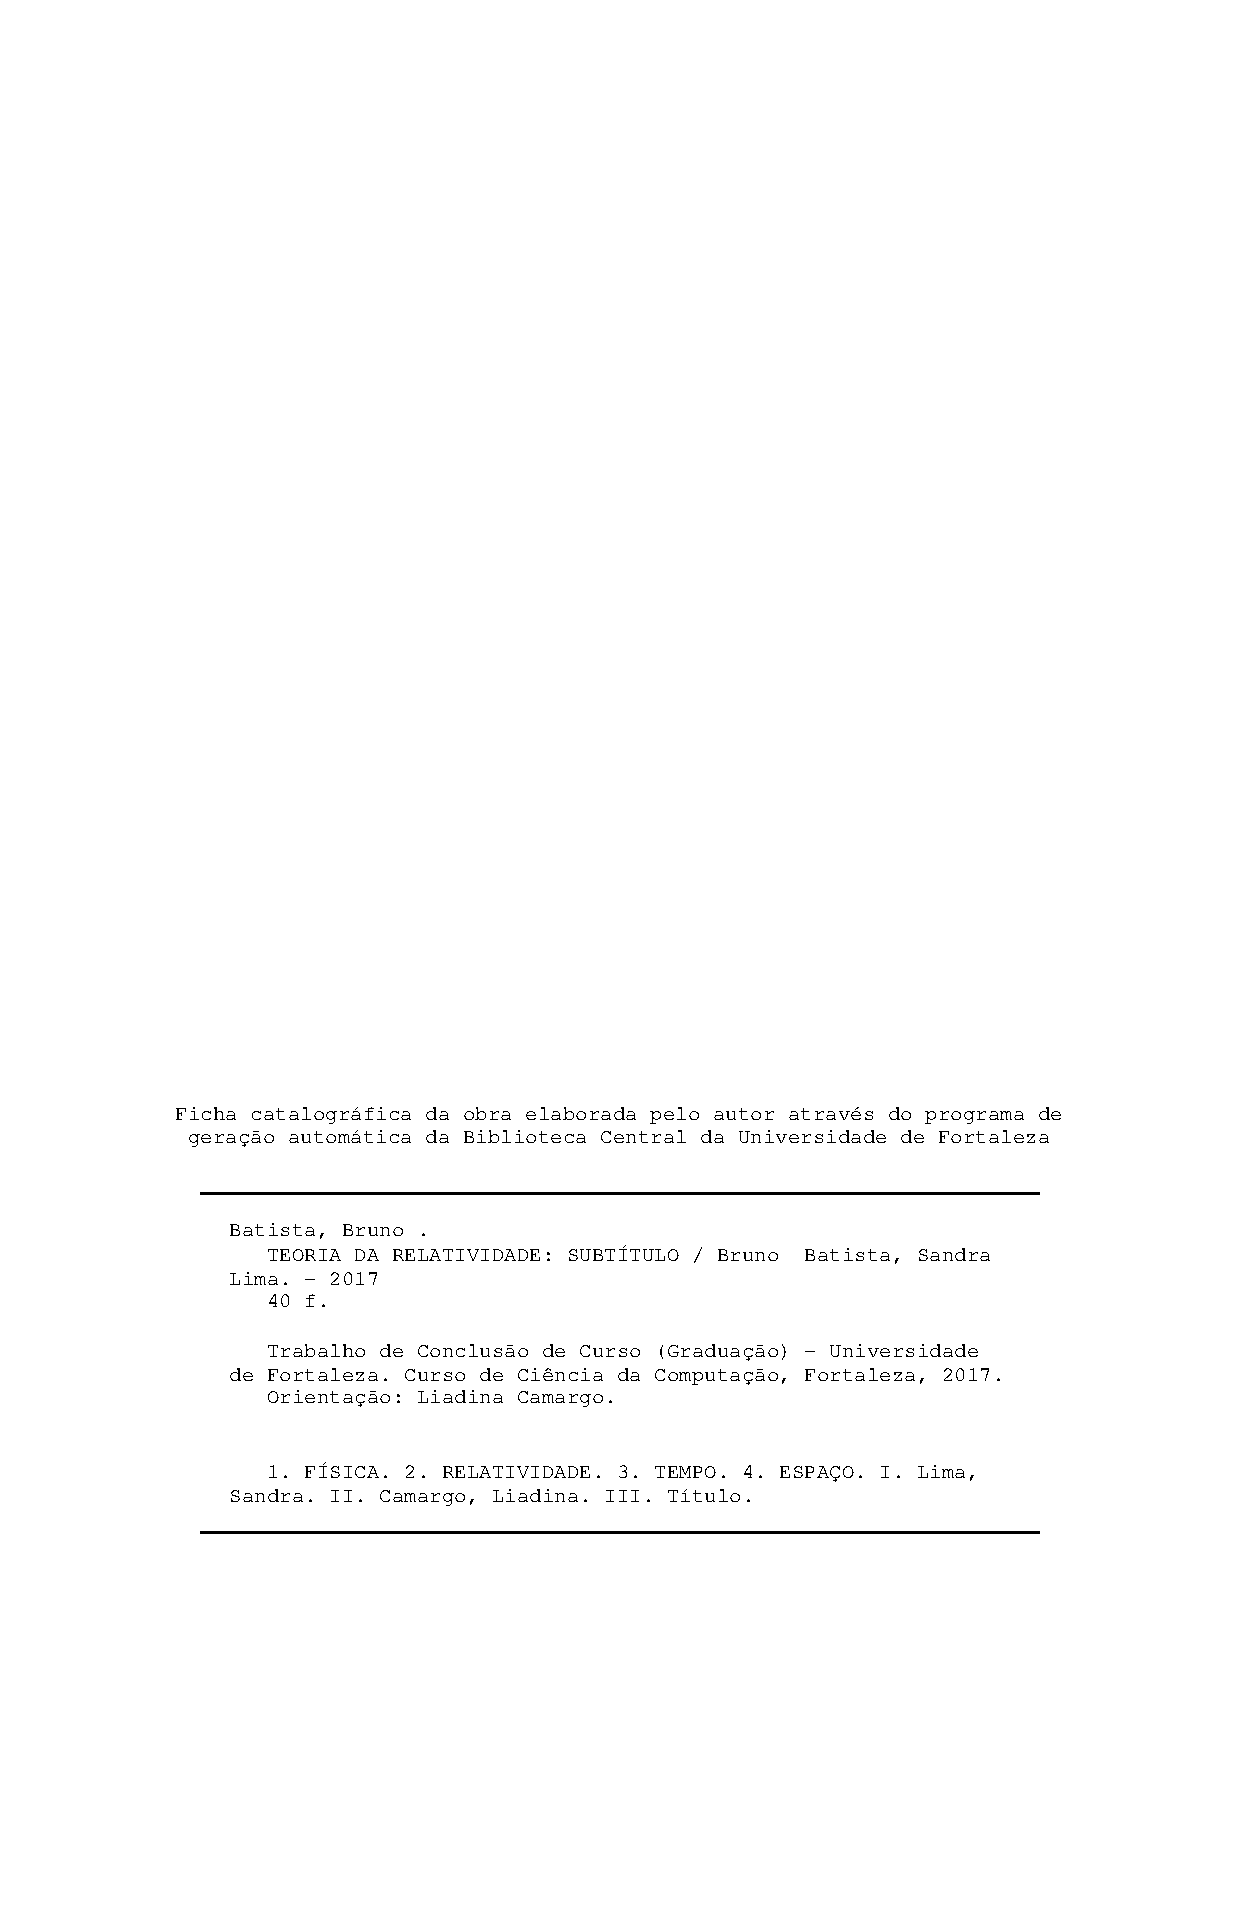
\includepdf{elementos-pre-textuais/folha-aprovacao.pdf}
		\imprimirfolhadeaprovacao

		\imprimirdedicatoria{elementos-pre-textuais/dedicatoria}
		\imprimiragradecimentos{elementos-pre-textuais/agradecimentos}
		\imprimirepigrafe{elementos-pre-textuais/epigrafe}
		\imprimirresumo{elementos-pre-textuais/resumo}
		\imprimirabstract{elementos-pre-textuais/abstract}
	\fi

	% Listas e sumário (comuns aos dois modos; cada lista sai vazia se o
	% documento não tiver o elemento correspondente).
	\imprimirlistadeilustracoes
	\imprimirlistadetabelas
	\imprimirlistadequadros
	\imprimirlistadealgoritmos
	\imprimirlistadecodigosfonte
	\imprimirlistadeabreviaturasesiglas
	\imprimirlistadesimbolos{elementos-pre-textuais/lista-de-simbolos}
	\imprimirsumario

	% Elementos textuais
	\textual
	\ifprobatorio
		%% --- Corpo do Relatório de Comprovação de Período Probatório ---
		%% A Seção 1 (Identificação) é gerada a partir dos metadados do servidor
		%% (\autor, \matriculasiape, \cargo, \lotacao, \periodoprobatorio, \chefia).
		\imprimiridentificacao
		%% >>> A PARTIR DAQUI, adicione os capítulos do SEU relatório. <<<
		%% A Seção 1.2 (entregas do plano de trabalho) e as Seções 2 a 8 são
		%% conteúdo seu: crie os arquivos em elementos-textuais/ e inclua-os com
		%% \input. Esqueleto sugerido (descomente e crie cada arquivo):
		%	\input{elementos-textuais/probatorio/entregas}            % 1.2
		%	\input{elementos-textuais/probatorio/contexto-objetivo}   % 2
		%	\input{elementos-textuais/probatorio/metodologia}         % 3
		%	\input{elementos-textuais/probatorio/comentarios-madeira} % 4
		%	\input{elementos-textuais/probatorio/comentarios-castanha}% 5
		%	\input{elementos-textuais/probatorio/analise-comparativa} % 6
		%	\input{elementos-textuais/probatorio/produtos-entregues}  % 7
		%	\input{elementos-textuais/probatorio/conclusao}           % 8
		%% Bloco de assinatura final (servidor + "De acordo" da chefia):
		\imprimirassinaturas
	\else
		%% >>> SEUS CAPÍTULOS — adicione/remova linhas \input conforme o seu
		%% documento (cada arquivo em elementos-textuais/ começa com \chapter). <<<
		\input{elementos-textuais/introducao}
		\input{elementos-textuais/revisao-de-literatura}
		\input{elementos-textuais/estado-da-arte}
		\input{elementos-textuais/material-e-metodos}
		\input{elementos-textuais/resultados-e-discussao}
		\input{elementos-textuais/consideracoes-finais}
	\fi

	% Elementos pós-textuais
	% Todos abaixo aparecem no PDF SOMENTE quando há conteúdo correspondente;
	% caso contrário, são omitidos automaticamente (sem título em página vazia).

	% Referências: impressas se houver \cite/\citeonline no texto. Para forçar
	% a inclusão de uma obra não citada (ex.: a norma ABNT NBR 14724), adicione
	% \nocite{NBR14724:2005} antes da linha abaixo.
	\imprimirreferencias{elementos-pos-textuais/referencias}

	% Glossário: impresso se algum termo do glossário principal for usado no
	% texto com \gls/\Gls (siglas vão para a Lista de Abreviaturas e Siglas).
	\imprimirglossario

	% Apêndices: passe os \input dentro das chaves. Deixe vazio para omitir.
	\imprimirapendices{%
		\input{elementos-pos-textuais/apendices/exemplo-de-apendice}%
	}

	% Anexos: passe os \input dentro das chaves. Deixe vazio para omitir.
	\imprimiranexos{%
		\input{elementos-pos-textuais/anexos/exemplo-de-anexo}%
	}

	% Índice remissivo: impresso apenas se houver entradas \index{} no texto.
	\imprimirindice

\end{document}
 —
% veja ./gerar-exemplos.sh. Na compilação normal, valem os padrões abaixo.

\providecommand{\TipoDoc}{publicacao}
\tipodocumento{\TipoDoc}

% Subtipo: cada tipo tem seu próprio seletor. Edite o valor do SEU tipo abaixo
% (só o seletor correspondente ao \TipoDoc escolhido é aplicado):
\providecommand{\Nivel}{relatorio}      % academico:   tcc | monografia | dissertacao | tese | relatorio
\providecommand{\Serie}{relatorio}      % publicacao:  relatorio | boletim | comunicado | documento
\providecommand{\Categoria}{relatorio}  % corporativo: relatorio | analise | probatorio
\ifacademico   \nivel{\Nivel}        \fi
\ifpublicacao  \serie{\Serie}        \fi
\ifcorporativo \categoria{\Categoria}\fi

% Caso não previsto? Defina os dois campos diretamente (é o que os seletores
% preenchem por baixo):
%   \subtitulodacapa{...}
%   \naturezadapublicacao{...}

% Remove as bordas vermelhas e verdes do PDF gerado
% Coloque 'sim' para remover

\removerbordasdohyperlink{sim}

% Adiciona a cor Azul a todos os hyperlinks

\cordohyperlink{nao}

%%%%%%%%%%%%%%%%%%%%%%%%%%%%%%%%%%%%%%%%%%%%%%%%%%%%%
%%       Informação sobre a Unidade Embrapa        %%
%%%%%%%%%%%%%%%%%%%%%%%%%%%%%%%%%%%%%%%%%%%%%%%%%%%%%

% Nome da unidade da Embrapa (ex.: Embrapa Agricultura Digital, Embrapa Cerrados, etc.)
% Em \providecommand para que os exemplos (exemplo-*.tex) o sobrescrevam via \def.
\providecommand{\Unidade}{Embrapa Agricultura Digital}
\unidade{\Unidade}
\providecommand{\UnidadeSigla}{CNPTIA}
\unidadesigla{\UnidadeSigla}

% Área ou centro de pesquisa (opcional)
\centro{}

%%%%%%%%%%%%%%%%%%%%%%%%%%%%%%%%%%%%%%%%%%%%%%%%%%%%%
%%   Informação acadêmica (tipo 'academico')       %%
%%%%%%%%%%%%%%%%%%%%%%%%%%%%%%%%%%%%%%%%%%%%%%%%%%%%%

% Campos usados no modo academico. Os \providecommand permitem que os exemplos
% (exemplo-*.tex) os sobrescrevam via \def; na compilação normal, edite os
% valores aqui.

% Instituição de ensino (universidade/IES). Usada na capa e no preâmbulo.
\providecommand{\Instituicao}{Embrapa Agricultura Digital}
\instituicao{\Instituicao}

% Programa de pós-graduação ou curso (compõe o preâmbulo em tcc/monografia/
% dissertacao/tese; não usado no nível 'relatorio').
\providecommand{\ProgramaPesquisa}{}
\programapesquisa{\ProgramaPesquisa}

% Aparecem na folha de rosto apenas se preenchidas (qualquer nível academico):
\providecommand{\AreaPesquisa}{}   % Área de concentração
\areadepesquisa{\AreaPesquisa}
\providecommand{\LinhaPesquisa}{}  % Linha de pesquisa
\linhapesquisa{\LinhaPesquisa}

%%%%%%%%%%%%%%%%%%%%%%%%%%%%%%%%%%%%%%%%%%%%%%%%%%%%%
%%   Informação da série (tipo 'publicacao')       %%
%%%%%%%%%%%%%%%%%%%%%%%%%%%%%%%%%%%%%%%%%%%%%%%%%%%%%

% Número do documento na série (ex.: 123). Impresso na capa se preenchido.
\providecommand{\NumeroDocumento}{}
\numerodocumento{\NumeroDocumento}

%%%%%%%%%%%%%%%%%%%%%%%%%%%%%%%%%%%%%%%%%%%%%%%%%%%%%
%%  Identificação do servidor (subtipo 'probatorio') %%
%%%%%%%%%%%%%%%%%%%%%%%%%%%%%%%%%%%%%%%%%%%%%%%%%%%%%

% Usados quando \TipoDoc{corporativo} + \Categoria{probatorio}. O NOME do
% servidor é o \autor (definido abaixo). Estes campos alimentam a Seção 1.1
% (\imprimiridentificacao) e o bloco de assinatura (\imprimirassinaturas).
% Deixe em branco ({}) os que não usar — somem da identificação automaticamente.
\providecommand{\MatriculaSiape}{}
\matriculasiape{\MatriculaSiape}
\providecommand{\Cargo}{}
\cargo{\Cargo}
\providecommand{\Lotacao}{}
\lotacao{\Lotacao}
\providecommand{\PeriodoProbatorio}{}
\periodoprobatorio{\PeriodoProbatorio}
\providecommand{\Chefia}{}            % Nome da chefia imediata (linha "De acordo")
\chefia{\Chefia}
\providecommand{\ChefiaCargo}{}       % Cargo/função da chefia imediata
\chefiacargo{\ChefiaCargo}

%%%%%%%%%%%%%%%%%%%%%%%%%%%%%%%%%%%%%%%%%%%%%%%%%%%%%
%%     Informação relacionada ao documento         %%
%%%%%%%%%%%%%%%%%%%%%%%%%%%%%%%%%%%%%%%%%%%%%%%%%%%%%

% Preencha com os dados do seu trabalho.
% Em \providecommand para que os exemplos (exemplo-*.tex) os sobrescrevam via \def.
\providecommand{\Autor}{Maria Exemplo da Silva}
\autor{\Autor}
\providecommand{\Titulo}{Análise de um Problema de Pesquisa: Um Estudo de Caso Ilustrativo}
\titulo{\Titulo}
\providecommand{\Data}{2026}
\data{\Data}
\providecommand{\Local}{Campinas -- SP}
\local{\Local}

% Data de aprovação (se aplicável). No subtipo 'probatorio' é a data de
% fechamento usada no bloco de assinatura.
% Exemplo: \dataaprovacao{01 de janeiro de 2026}
\providecommand{\DataAprovacao}{15 de junho de 2026}
\dataaprovacao{\DataAprovacao}

%%%%%%%%%%%%%%%%%%%%%%%%%%%%%%%%%%%%%%%%%%%%%%%%%%%%%
%%     Informação sobre o Orientador/Supervisor    %%
%%%%%%%%%%%%%%%%%%%%%%%%%%%%%%%%%%%%%%%%%%%%%%%%%%%%%

% Orientador/supervisor (modo academico). Em \providecommand para os exemplos
% sobrescreverem; vazio por padrão — num publicacao/relatorio não há orientador.
\providecommand{\Orientador}{}
\orientador{\Orientador}
\providecommand{\OrientadorIes}{}
\orientadories{\OrientadorIes}
\orientadorcentro{}
\orientadorfeminino{nao} % Coloque 'sim' se for do sexo feminino

%%%%%%%%%%%%%%%%%%%%%%%%%%%%%%%%%%%%%%%%%%%%%%%%%%%%%
%%      Informação sobre o Co-orientador           %%
%%%%%%%%%%%%%%%%%%%%%%%%%%%%%%%%%%%%%%%%%%%%%%%%%%%%%

% Deixe o nome do coorientador em branco para remover do documento

\coorientador{}
\coorientadories{}
\coorientadorcentro{}
\coorientadorfeminino{nao} % Coloque 'sim' se for do sexo feminino

%%%%%%%%%%%%%%%%%%%%%%%%%%%%%%%%%%%%%%%%%%%%%%%%%%%%%
%%      Informação sobre a banca/revisores         %%
%%%%%%%%%%%%%%%%%%%%%%%%%%%%%%%%%%%%%%%%%%%%%%%%%%%%%

% Deixe o nome do membro em branco para remover da folha de aprovação
% Exemplo de uso:
% \membrodabancadois{Dr. Fulano de Tal}
% \membrodabancadoisies{Embrapa Cerrados}

\providecommand{\MembroBancaDois}{}
\membrodabancadois{\MembroBancaDois}
\membrodabancadoiscentro{}
\providecommand{\MembroBancaDoisIes}{}
\membrodabancadoisies{\MembroBancaDoisIes}

\providecommand{\MembroBancaTres}{}
\membrodabancatres{\MembroBancaTres}
\membrodabancatrescentro{}
\providecommand{\MembroBancaTresIes}{}
\membrodabancatresies{\MembroBancaTresIes}

\membrodabancaquatro{}
\membrodabancaquatrocentro{}
\membrodabancaquatroies{}

\membrodabancacinco{}
\membrodabancacincocentro{}
\membrodabancacincoies{}

\membrodabancaseis{}
\membrodabancaseiscentro{}
\membrodabancaseisies{}

%%%%%%%%%%%%%%%%%%%%%%%%%%%%%%%%%%%%%%%%%%%%%%%%%%%%%
%%        Informação da Ficha Catalográfica        %%
%%%%%%%%%%%%%%%%%%%%%%%%%%%%%%%%%%%%%%%%%%%%%%%%%%%%%

% A ficha catalográfica é gerada automaticamente em LaTeX a partir dos campos
% abaixo — não é mais necessário anexar um PDF externo. Os dados de
% classificação (CDD/CDU), os descritores de assunto e o registro CRB do
% bibliotecário devem ser fornecidos por um(a) bibliotecário(a).

% Nome do autor invertido para a entrada principal (Sobrenome, Nome).
% Se ficar em branco, será usado o \autor definido acima.
\autorinvertido{Silva, Maria Exemplo da}

% Dados da publicação
\edicao{1. ed.}           % Ex.: 1. ed. (deixe em branco se não houver)
\editora{Embrapa}         % Editora responsável
\numeropaginas{30}        % Número total de páginas (ex.: 85)
\ilustracao{il. color.}   % Ex.: il. / il. color. (deixe em branco se não houver)
\dimensao{21 cm}          % Altura da publicação

% Informações complementares
\isbn{978-65-00000-00-0}  % ISBN, se houver
\notaficha{Documento de exemplo gerado com o template EmbrapaTex.} % Nota livre (ex.: tipo do trabalho, orientador)
\incluibibliografia{sim}  % 'sim' imprime "Inclui bibliografia."

% Dados fornecidos pelo(a) bibliotecário(a)
\descritores{1. Pesquisa. 2. Metodologia científica. 3. Documentação técnica. I. Título.} % Ex.: 1. Agricultura digital. 2. Sensoriamento remoto. I. Título.
\cdd{001.42}              % Classificação Decimal de Dewey (ex.: 630)
\cdu{}                    % Classificação Decimal Universal (opcional)
\bibliotecario{Bibliotecário(a) Exemplo} % Nome do(a) bibliotecário(a)
\crb{CRB-8/0000}          % Registro profissional (ex.: CRB-1/1234)

%%%%%%%%%%%%%%%%%%%%%%%%%%%%%%%%%%%%%%%%%%%%%%%%%%%%%%%%%%%%%%%%%%%%%%%%
%% >>> SEUS DADOS (fim) <<<
%% Daqui para baixo é a ESTRUTURA do documento (montagem automática:
%% capa, folha de rosto, listas, sumário, referências, apêndices...).
%% Normalmente você só precisa editar a LISTA DE CAPÍTULOS — procure
%% por "SEUS CAPÍTULOS" mais abaixo.
%%%%%%%%%%%%%%%%%%%%%%%%%%%%%%%%%%%%%%%%%%%%%%%%%%%%%%%%%%%%%%%%%%%%%%%%
\begin{document}

	% Elementos pré-textuais
	\imprimircapa
	\imprimirfolhaderosto

	%%%%%%%%%%%%%%%%%%%%%%%%%%%%%%%%%%%%%%%%%%%%%%%%%%%%%%%%%%%%%%%%%%%%%%%%%%
	%%  Os elementos pré-textuais variam conforme \tipodocumento:           %%
	%%   - corporativo  -> sumário executivo (modo empresarial)             %%
	%%   - demais tipos -> estrutura acadêmica/ABNT completa                %%
	%%  O condicional \ifcorporativo é definido em lib/embrapatex.sty.      %%
	%%%%%%%%%%%%%%%%%%%%%%%%%%%%%%%%%%%%%%%%%%%%%%%%%%%%%%%%%%%%%%%%%%%%%%%%%%
	\ifcorporativo
		%% ----- Modo corporativo/empresarial -----
		\imprimirsumarioexecutivo{elementos-pre-textuais/sumario-executivo}
	\else
		%% ----- Modo acadêmico/científico (ABNT) -----
		\imprimirfichacatalografica
		\imprimirerrata{elementos-pre-textuais/errata}

		%%%%%%%%%%%%%%%%%%%%%%%%%%%%%%%%%%%%%%%%%%%%%%%%%%%%%%%%%%%%%%%%%%%%%%
		%%  Folha de aprovação:                                             %%
		%%  Caso possua uma folha de aprovação assinada em PDF,             %%
		%%  descomente a linha \includepdf abaixo e comente                 %%
		%%  a linha \imprimirfolhadeaprovacao.                              %%
		%%%%%%%%%%%%%%%%%%%%%%%%%%%%%%%%%%%%%%%%%%%%%%%%%%%%%%%%%%%%%%%%%%%%%%

		%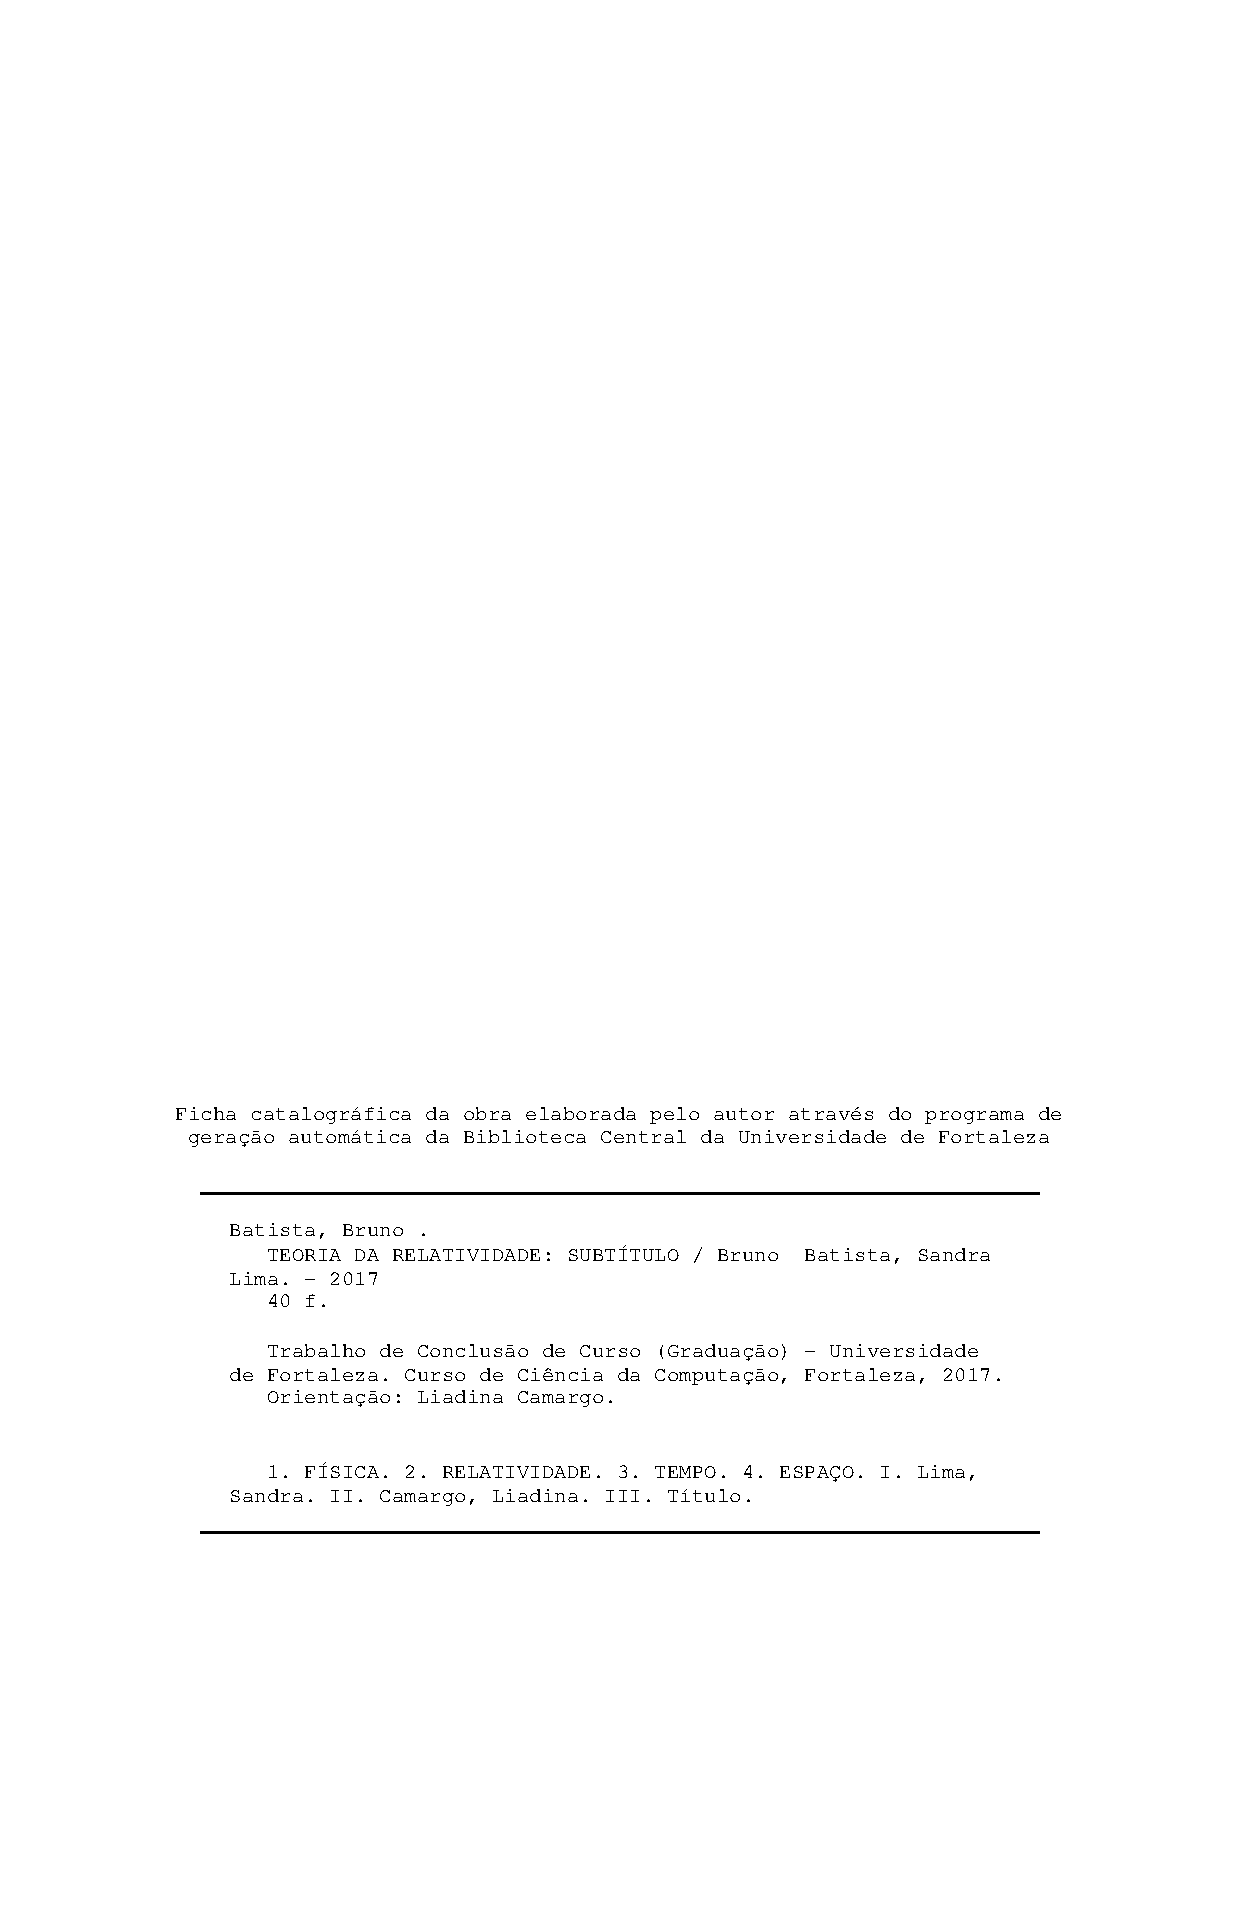
\includepdf{elementos-pre-textuais/folha-aprovacao.pdf}
		\imprimirfolhadeaprovacao

		\imprimirdedicatoria{elementos-pre-textuais/dedicatoria}
		\imprimiragradecimentos{elementos-pre-textuais/agradecimentos}
		\imprimirepigrafe{elementos-pre-textuais/epigrafe}
		\imprimirresumo{elementos-pre-textuais/resumo}
		\imprimirabstract{elementos-pre-textuais/abstract}
	\fi

	% Listas e sumário (comuns aos dois modos; cada lista sai vazia se o
	% documento não tiver o elemento correspondente).
	\imprimirlistadeilustracoes
	\imprimirlistadetabelas
	\imprimirlistadequadros
	\imprimirlistadealgoritmos
	\imprimirlistadecodigosfonte
	\imprimirlistadeabreviaturasesiglas
	\imprimirlistadesimbolos{elementos-pre-textuais/lista-de-simbolos}
	\imprimirsumario

	% Elementos textuais
	\textual
	\ifprobatorio
		%% --- Corpo do Relatório de Comprovação de Período Probatório ---
		%% A Seção 1 (Identificação) é gerada a partir dos metadados do servidor
		%% (\autor, \matriculasiape, \cargo, \lotacao, \periodoprobatorio, \chefia).
		\imprimiridentificacao
		%% >>> A PARTIR DAQUI, adicione os capítulos do SEU relatório. <<<
		%% A Seção 1.2 (entregas do plano de trabalho) e as Seções 2 a 8 são
		%% conteúdo seu: crie os arquivos em elementos-textuais/ e inclua-os com
		%% \input. Esqueleto sugerido (descomente e crie cada arquivo):
		%	\input{elementos-textuais/probatorio/entregas}            % 1.2
		%	\input{elementos-textuais/probatorio/contexto-objetivo}   % 2
		%	\input{elementos-textuais/probatorio/metodologia}         % 3
		%	\input{elementos-textuais/probatorio/comentarios-madeira} % 4
		%	\input{elementos-textuais/probatorio/comentarios-castanha}% 5
		%	\input{elementos-textuais/probatorio/analise-comparativa} % 6
		%	\input{elementos-textuais/probatorio/produtos-entregues}  % 7
		%	\input{elementos-textuais/probatorio/conclusao}           % 8
		%% Bloco de assinatura final (servidor + "De acordo" da chefia):
		\imprimirassinaturas
	\else
		%% >>> SEUS CAPÍTULOS — adicione/remova linhas \input conforme o seu
		%% documento (cada arquivo em elementos-textuais/ começa com \chapter). <<<
		\chapter{Introdução}
\label{cap:introducao}

% Descreva aqui o contexto geral do trabalho, apresentando o tema,
% a problemática e a justificativa da pesquisa.

% [Insira o texto da introdução aqui]
O avanço do conhecimento científico depende, em grande medida, da capacidade de organizar e comunicar resultados de forma clara e padronizada. Instituições de pesquisa como a \gls{EMBRAPA} desempenham papel fundamental nesse processo, ao gerar e difundir conhecimento aplicado a diversos setores, entre eles o da \gls{agropecuaria}. Este documento apresenta, de maneira genérica, a estrutura típica de um trabalho técnico-científico, com o objetivo de demonstrar a formatação adotada pelo template, cujo documento final é gerado em formato \gls{PDF}.

\section{Justificativa}
\label{sec:justificativa}

% Apresente a relevância e a motivação para a realização deste trabalho.

% [Insira a justificativa aqui]
A escolha do tema justifica-se por sua relevância teórica e prática, bem como pela necessidade de aprofundar a compreensão sobre o assunto. A realização deste estudo contribui para preencher lacunas identificadas na literatura e para fornecer subsídios a futuras investigações e aplicações.

\section{Objetivos}
\label{sec:objetivos}

% Apresente os objetivos geral e específicos do trabalho.

\subsection{Objetivo Geral}
\label{sec:objetivo-geral}

% [Insira o objetivo geral aqui]
Investigar de forma sistemática os fatores associados ao problema em estudo, com vistas a ampliar o conhecimento disponível sobre o tema.

\subsection{Objetivos Específicos}
\label{sec:objetivos-especificos}

% Liste os objetivos específicos usando alíneas:
%
% \begin{alineas}
% 	\item Objetivo específico 1;
% 	\item Objetivo específico 2;
% 	\item Objetivo específico 3.
% \end{alineas}

% [Insira os objetivos específicos aqui]
Para alcançar o objetivo geral, foram definidos os seguintes objetivos específicos:

\begin{alineas}
	\item revisar a literatura pertinente ao tema investigado;
	\item descrever os procedimentos metodológicos adotados;
	\item analisar os dados obtidos e discutir os resultados;
	\item apresentar conclusões e recomendações para trabalhos futuros.
\end{alineas}
		\chapter{Revisão de Literatura}
\label{cap:revisao-de-literatura}

% Apresente aqui a fundamentação teórica do trabalho.
% Realize uma revisão bibliográfica dos principais conceitos,
% teorias e trabalhos anteriores relacionados ao tema.

% [Insira o texto da revisão de literatura aqui]
A fundamentação teórica deste trabalho apoia-se em contribuições consolidadas na literatura. De acordo com \citeonline{exemplo-livro}, os conceitos fundamentais que norteiam a área foram estabelecidos a partir de investigações sistemáticas conduzidas ao longo das últimas décadas. Estudos posteriores ampliaram essa compreensão, agregando novas perspectivas ao debate~\cite{exemplo-artigo}.

\section{Tema A}
\label{sec:tema-a}

% [Insira o conteúdo da primeira seção aqui]
Esta seção apresenta os principais conceitos relacionados ao primeiro eixo temático do estudo. A \autoref{fig:exemplo} ilustra, a título de demonstração, uma figura inserida conforme o padrão do template.

\begin{figure}[!htbp]
    \centering
    \EMBRAPAfig{
        \Caption{\label{fig:exemplo} Exemplo de figura inserida com o template}
    }{
        
\includegraphics[width=10cm]{figuras/exemplo_imagem.jpg}
    }{
        \Fonte{Embrapa}
    }
\end{figure}

% Dica: Para inserir uma figura, use o seguinte modelo:
%
% \begin{figure}[!htbp]
%     \centering
%     \EMBRAPAfig{
%         \Caption{\label{fig:modelo} Legenda da figura}
%     }{
%         \includegraphics[width=8cm]{figuras/nome-da-figura}
%     }{
%         \Fonte{Elaborado pelo autor}
%     }
% \end{figure}

\section{Tema B}
\label{sec:tema-b}

% [Insira o conteúdo da segunda seção aqui]
O segundo eixo temático complementa a discussão anterior, abordando aspectos adicionais relevantes para a compreensão do problema. A literatura registra convergências e divergências entre os autores, o que evidencia a riqueza e a complexidade do tema.

% Dica: Para inserir uma tabela, use o seguinte modelo:
%
% \begin{table}[!htbp]
%     \centering
%     \Caption{\label{tab:exemplo} Legenda da tabela}
%     \EMBRAPAtab{}{
%         \begin{tabular}{cll}
%             \toprule
%             Coluna 1 & Coluna 2 & Coluna 3 \\
%             \midrule \midrule
%             Dado 1 & Dado 2 & Dado 3 \\
%             \bottomrule
%         \end{tabular}
%     }{
%         \Fonte{Elaborado pelo autor}
%     }
% \end{table}

		\chapter{Estado da Arte}
\label{cap:estado-da-arte}

% Apresente aqui uma revisão dos trabalhos e pesquisas mais recentes
% relacionados ao tema, destacando as contribuições e lacunas existentes.

% [Insira o texto do estado da arte aqui]
Esta seção apresenta uma síntese dos trabalhos mais recentes relacionados ao tema, com destaque para suas contribuições e para as lacunas ainda existentes.

\section{Trabalho/Pesquisa A}
\label{sec:trabalho-a}

% [Descreva o primeiro trabalho relacionado]
O primeiro trabalho analisado propõe uma abordagem inovadora para o problema, apresentando resultados promissores em cenários controlados.

\section{Trabalho/Pesquisa B}
\label{sec:trabalho-b}

% [Descreva o segundo trabalho relacionado]
O segundo trabalho, por sua vez, adota uma estratégia distinta, privilegiando a generalização dos resultados. O \autoref{qua:comparativo} sintetiza a comparação entre as duas abordagens.

\begin{quadro}[!htbp]
    \centering
    \Caption{\label{qua:comparativo} Comparação entre as abordagens analisadas}
    \EMBRAPAqua{}{
        \begin{tabular}{|l|c|c|}
            \hline
            \textbf{Critério} & \textbf{Trabalho A} & \textbf{Trabalho B} \\
            \hline
            Abordagem & Inovadora & Tradicional \\
            \hline
            Escopo & Restrito & Amplo \\
            \hline
            Desempenho & Alto & Moderado \\
            \hline
        \end{tabular}
    }{
        \Fonte{Elaborado pelo autor}
    }
\end{quadro}

% Dica: Para inserir um quadro comparativo, use o seguinte modelo:
%
% \begin{quadro}[!htbp]
%     \centering
%     \Caption{\label{qua:modelo} Legenda do quadro}
%     \EMBRAPAqua{}{
%         \begin{tabular}{|c|c|c|}
%             \hline
%             Critério & Trabalho A & Trabalho B \\
%             \hline
%             Critério 1 & Valor & Valor \\
%             \hline
%         \end{tabular}
%     }{
%         \Fonte{Elaborado pelo autor}
%     }
% \end{quadro}

		\chapter{Material e Métodos}
\label{cap:material-e-metodos}

% Descreva aqui os materiais utilizados e os métodos empregados
% na realização da pesquisa. Inclua informações sobre:
% - Área de estudo / local do experimento
% - Materiais e equipamentos
% - Delineamento experimental
% - Procedimentos analíticos
% - Análises estatísticas

% [Insira o texto de material e métodos aqui]
Este capítulo descreve os materiais e os métodos empregados na condução do estudo. A apresentação segue as recomendações da \gls{ABNT}, de modo a assegurar a padronização e a reprodutibilidade dos procedimentos.

\section{Área de Estudo}
\label{sec:area-de-estudo}

% [Descreva a área ou local onde o trabalho foi realizado]
O estudo foi conduzido em ambiente representativo do contexto investigado, selecionado de acordo com critérios previamente definidos.

\section{Procedimentos Metodológicos}
\label{sec:procedimentos-metodologicos}

% [Descreva os procedimentos utilizados]
Os procedimentos adotados são sintetizados no \autoref{alg:exemplo}, que descreve, em alto nível, as etapas executadas ao longo do estudo.

\begin{algorithm}[!htbp]
    \SetSpacedAlgorithm
    \caption{\label{alg:exemplo}Procedimento geral adotado no estudo}
    \Entrada{Conjunto de dados brutos $D$}
    \Saida{Resultados consolidados $R$}
    \Inicio{
        \Para{cada elemento $d \in D$}{
            processar $d$\;
            armazenar o resultado parcial\;
        }
        consolidar os resultados em $R$\;
        \Retorna $R$\;
    }
\end{algorithm}

% Dica: Para inserir um algoritmo, use o seguinte modelo:
%
% \begin{algorithm}[h!]
%     \SetSpacedAlgorithm
%     \caption{\label{alg:modelo}Descrição do Algoritmo}
%     \Entrada{Entrada do Algoritmo}
%     \Saida{Saída do Algoritmo}
%     \Inicio{
%         Passo 1\;
%         Passo 2\;
%     }
% \end{algorithm}

\section{Análise dos Dados}
\label{sec:analise-dos-dados}

% [Descreva como os dados foram analisados]
Os dados foram analisados por meio de procedimentos estatísticos descritivos e inferenciais. A relação entre as variáveis é expressa, de forma simplificada, pela \autoref{eq:modelo}.

\begin{equation}
    \label{eq:modelo}
    y = ax + b
\end{equation}

\noindent onde $y$ representa a variável resposta, $x$ a variável explicativa, e $a$ e $b$ os coeficientes do modelo.

Para a inferência sobre a média populacional $\mu$, adotou-se o nível de significância $\alpha$ e construiu-se o intervalo de confiança a partir do desvio-padrão $\sigma$ e do tamanho da amostra $n$, conforme a \autoref{eq:intervalo}.

\begin{equation}
    \label{eq:intervalo}
    \mu = \bar{x} \pm z_{\alpha/2}\,\frac{\sigma}{\sqrt{n}}
\end{equation}

% Dica: Para inserir uma fórmula matemática numerada e referenciável:
%
% \begin{equation}
%     \label{eq:exemplo}
%     y = ax + b
% \end{equation}
%
% Referencie no texto com \autoref{eq:exemplo} (ou \autoref{sec:area-de-estudo}).

		\chapter{Resultados e Discussão}
\label{cap:resultados-e-discussao}

% Apresente aqui os resultados obtidos na pesquisa e discuta-os
% à luz da literatura revisada. Inclua figuras, tabelas e gráficos
% conforme necessário.

% [Insira os resultados e a discussão aqui]
Este capítulo apresenta os resultados obtidos e discute suas implicações à luz da literatura revisada.

\section{Resultados}
\label{sec:resultados}

% [Apresente os resultados obtidos]
Os principais resultados são apresentados na \autoref{tab:resultados}, que sintetiza os valores observados para as variáveis analisadas.

\begin{table}[!htbp]
    \centering
    \Caption{\label{tab:resultados} Síntese dos resultados obtidos}
    \EMBRAPAtab{}{
        \begin{tabular}{lcc}
            \toprule
            Variável & Valor médio & Desvio-padrão \\
            \midrule \midrule
            Indicador A & 12,5 & 1,3 \\
            Indicador B & 8,7 & 0,9 \\
            Indicador C & 21,4 & 2,1 \\
            \bottomrule
        \end{tabular}
    }{
        \Fonte{Elaborado pelo autor}
    }
\end{table}

\section{Discussão}
\label{sec:discussao}

% [Discuta os resultados à luz da literatura]
Os resultados obtidos são coerentes com as expectativas formuladas e dialogam com os achados relatados na literatura. As pequenas divergências observadas podem ser atribuídas a particularidades do contexto investigado e apontam direções para estudos futuros.

		\chapter{Considerações Finais}
\label{cap:consideracoes-finais}

% Apresente aqui as conclusões do trabalho, retomando os objetivos
% propostos e avaliando se foram alcançados.

% [Insira as considerações finais aqui]
Este trabalho buscou investigar de forma sistemática o problema proposto, retomando os objetivos definidos na introdução e avaliando em que medida foram alcançados.

\section{Contribuições do Trabalho}
\label{sec:contribuicoes-do-trabalho}

% [Descreva as principais contribuições]
Entre as principais contribuições do estudo, destacam-se a sistematização do conhecimento sobre o tema e a proposição de subsídios para aplicações práticas.

\section{Limitações}
\label{sec:limitacoes}

% [Descreva as limitações encontradas]
Como toda investigação, este trabalho apresenta limitações, sobretudo quanto ao escopo e às condições em que foi conduzido, o que deve ser considerado na interpretação dos resultados.

\section{Recomendações e Trabalhos Futuros}
\label{sec:recomendacoes-e-trabalhos-futuros}

% [Apresente recomendações e sugestões para trabalhos futuros]
Recomenda-se, para trabalhos futuros, a ampliação do escopo da análise e a investigação de novas variáveis, de modo a consolidar e generalizar os achados aqui apresentados.

	\fi

	% Elementos pós-textuais
	% Todos abaixo aparecem no PDF SOMENTE quando há conteúdo correspondente;
	% caso contrário, são omitidos automaticamente (sem título em página vazia).

	% Referências: impressas se houver \cite/\citeonline no texto. Para forçar
	% a inclusão de uma obra não citada (ex.: a norma ABNT NBR 14724), adicione
	% \nocite{NBR14724:2005} antes da linha abaixo.
	\imprimirreferencias{elementos-pos-textuais/referencias}

	% Glossário: impresso se algum termo do glossário principal for usado no
	% texto com \gls/\Gls (siglas vão para a Lista de Abreviaturas e Siglas).
	\imprimirglossario

	% Apêndices: passe os \input dentro das chaves. Deixe vazio para omitir.
	\imprimirapendices{%
		\apendice{Exemplo de Apêndice}
\label{ap:exemplo-de-apendice}

% Apêndice é um texto ou documento elaborado pelo autor.
% Adicione aqui o conteúdo do apêndice.

Este apêndice apresenta material complementar elaborado pelo autor, como dados adicionais, formulários ou detalhamentos que apoiam o texto principal sem comprometer a sua fluidez.

% Tabela LONGA (multipágina): use o ambiente \EMBRAPAtablonga, que quebra entre
% páginas e repete o cabeçalho automaticamente. Ao contrário de \EMBRAPAtab, ele
% NÃO vai dentro de um ambiente 'table'. Os argumentos são, na ordem: colunas do
% tabular, legenda (com \label), linha de cabeçalho e texto da fonte. Veja o
% README ("Como inserir uma Tabela longa") e o CLAUDE.md.
\begin{EMBRAPAtablonga}{lrr}{\label{tab:apendice-amostras} Resultados de análise das amostras de solo coletadas (dados fictícios)}{Amostra & pH em água & Matéria orgânica (g/kg)}{Elaborado pelo autor}
	Amostra 001 & 5,3 & 21 \\
	Amostra 002 & 6,6 & 28 \\
	Amostra 003 & 4,9 & 35 \\
	Amostra 004 & 5,2 & 42 \\
	Amostra 005 & 6,5 & 17 \\
	Amostra 006 & 4,8 & 24 \\
	Amostra 007 & 5,1 & 31 \\
	Amostra 008 & 6,4 & 38 \\
	Amostra 009 & 4,7 & 45 \\
	Amostra 010 & 5,0 & 20 \\
	Amostra 011 & 6,3 & 27 \\
	Amostra 012 & 4,6 & 34 \\
	Amostra 013 & 5,9 & 41 \\
	Amostra 014 & 6,2 & 16 \\
	Amostra 015 & 4,5 & 23 \\
	Amostra 016 & 5,8 & 30 \\
	Amostra 017 & 6,1 & 37 \\
	Amostra 018 & 4,4 & 44 \\
	Amostra 019 & 5,7 & 19 \\
	Amostra 020 & 6,0 & 26 \\
	Amostra 021 & 4,3 & 33 \\
	Amostra 022 & 5,6 & 40 \\
	Amostra 023 & 6,9 & 15 \\
	Amostra 024 & 4,2 & 22 \\
	Amostra 025 & 5,5 & 29 \\
	Amostra 026 & 6,8 & 36 \\
	Amostra 027 & 4,1 & 43 \\
	Amostra 028 & 5,4 & 18 \\
	Amostra 029 & 6,7 & 25 \\
	Amostra 030 & 4,0 & 32 \\
	Amostra 031 & 5,3 & 39 \\
	Amostra 032 & 6,6 & 14 \\
	Amostra 033 & 4,9 & 21 \\
	Amostra 034 & 5,2 & 28 \\
	Amostra 035 & 6,5 & 35 \\
	Amostra 036 & 4,8 & 42 \\
	Amostra 037 & 5,1 & 17 \\
	Amostra 038 & 6,4 & 24 \\
	Amostra 039 & 4,7 & 31 \\
	Amostra 040 & 5,0 & 38 \\
\end{EMBRAPAtablonga}
%
	}

	% Anexos: passe os \input dentro das chaves. Deixe vazio para omitir.
	\imprimiranexos{%
		\anexo{Exemplo de Anexo}
\label{an:exemplo-de-anexo}

% Anexo é um texto ou documento não elaborado pelo autor.
% Adicione aqui o conteúdo do anexo.

% [Insira o conteúdo do anexo aqui]
Este anexo reúne material de apoio não elaborado pelo autor, como documentos, tabelas ou normas de terceiros que complementam o conteúdo do trabalho.%
	}

	% Índice remissivo: impresso apenas se houver entradas \index{} no texto.
	\imprimirindice

\end{document}
 —
% veja ./gerar-exemplos.sh. Na compilação normal, valem os padrões abaixo.

\providecommand{\TipoDoc}{publicacao}
\tipodocumento{\TipoDoc}

% Subtipo: cada tipo tem seu próprio seletor. Edite o valor do SEU tipo abaixo
% (só o seletor correspondente ao \TipoDoc escolhido é aplicado):
\providecommand{\Nivel}{relatorio}      % academico:   tcc | monografia | dissertacao | tese | relatorio
\providecommand{\Serie}{relatorio}      % publicacao:  relatorio | boletim | comunicado | documento
\providecommand{\Categoria}{relatorio}  % corporativo: relatorio | analise | probatorio
\ifacademico   \nivel{\Nivel}        \fi
\ifpublicacao  \serie{\Serie}        \fi
\ifcorporativo \categoria{\Categoria}\fi

% Caso não previsto? Defina os dois campos diretamente (é o que os seletores
% preenchem por baixo):
%   \subtitulodacapa{...}
%   \naturezadapublicacao{...}

% Remove as bordas vermelhas e verdes do PDF gerado
% Coloque 'sim' para remover

\removerbordasdohyperlink{sim}

% Adiciona a cor Azul a todos os hyperlinks

\cordohyperlink{nao}

%%%%%%%%%%%%%%%%%%%%%%%%%%%%%%%%%%%%%%%%%%%%%%%%%%%%%
%%       Informação sobre a Unidade Embrapa        %%
%%%%%%%%%%%%%%%%%%%%%%%%%%%%%%%%%%%%%%%%%%%%%%%%%%%%%

% Nome da unidade da Embrapa (ex.: Embrapa Agricultura Digital, Embrapa Cerrados, etc.)
% Em \providecommand para que os exemplos (exemplo-*.tex) o sobrescrevam via \def.
\providecommand{\Unidade}{Embrapa Agricultura Digital}
\unidade{\Unidade}
\providecommand{\UnidadeSigla}{CNPTIA}
\unidadesigla{\UnidadeSigla}

% Área ou centro de pesquisa (opcional)
\centro{}

%%%%%%%%%%%%%%%%%%%%%%%%%%%%%%%%%%%%%%%%%%%%%%%%%%%%%
%%   Informação acadêmica (tipo 'academico')       %%
%%%%%%%%%%%%%%%%%%%%%%%%%%%%%%%%%%%%%%%%%%%%%%%%%%%%%

% Campos usados no modo academico. Os \providecommand permitem que os exemplos
% (exemplo-*.tex) os sobrescrevam via \def; na compilação normal, edite os
% valores aqui.

% Instituição de ensino (universidade/IES). Usada na capa e no preâmbulo.
\providecommand{\Instituicao}{Embrapa Agricultura Digital}
\instituicao{\Instituicao}

% Programa de pós-graduação ou curso (compõe o preâmbulo em tcc/monografia/
% dissertacao/tese; não usado no nível 'relatorio').
\providecommand{\ProgramaPesquisa}{}
\programapesquisa{\ProgramaPesquisa}

% Aparecem na folha de rosto apenas se preenchidas (qualquer nível academico):
\providecommand{\AreaPesquisa}{}   % Área de concentração
\areadepesquisa{\AreaPesquisa}
\providecommand{\LinhaPesquisa}{}  % Linha de pesquisa
\linhapesquisa{\LinhaPesquisa}

%%%%%%%%%%%%%%%%%%%%%%%%%%%%%%%%%%%%%%%%%%%%%%%%%%%%%
%%   Informação da série (tipo 'publicacao')       %%
%%%%%%%%%%%%%%%%%%%%%%%%%%%%%%%%%%%%%%%%%%%%%%%%%%%%%

% Número do documento na série (ex.: 123). Impresso na capa se preenchido.
\providecommand{\NumeroDocumento}{}
\numerodocumento{\NumeroDocumento}

%%%%%%%%%%%%%%%%%%%%%%%%%%%%%%%%%%%%%%%%%%%%%%%%%%%%%
%%  Identificação do servidor (subtipo 'probatorio') %%
%%%%%%%%%%%%%%%%%%%%%%%%%%%%%%%%%%%%%%%%%%%%%%%%%%%%%

% Usados quando \TipoDoc{corporativo} + \Categoria{probatorio}. O NOME do
% servidor é o \autor (definido abaixo). Estes campos alimentam a Seção 1.1
% (\imprimiridentificacao) e o bloco de assinatura (\imprimirassinaturas).
% Deixe em branco ({}) os que não usar — somem da identificação automaticamente.
\providecommand{\MatriculaSiape}{}
\matriculasiape{\MatriculaSiape}
\providecommand{\Cargo}{}
\cargo{\Cargo}
\providecommand{\Lotacao}{}
\lotacao{\Lotacao}
\providecommand{\PeriodoProbatorio}{}
\periodoprobatorio{\PeriodoProbatorio}
\providecommand{\Chefia}{}            % Nome da chefia imediata (linha "De acordo")
\chefia{\Chefia}
\providecommand{\ChefiaCargo}{}       % Cargo/função da chefia imediata
\chefiacargo{\ChefiaCargo}

%%%%%%%%%%%%%%%%%%%%%%%%%%%%%%%%%%%%%%%%%%%%%%%%%%%%%
%%     Informação relacionada ao documento         %%
%%%%%%%%%%%%%%%%%%%%%%%%%%%%%%%%%%%%%%%%%%%%%%%%%%%%%

% Preencha com os dados do seu trabalho.
% Em \providecommand para que os exemplos (exemplo-*.tex) os sobrescrevam via \def.
\providecommand{\Autor}{Maria Exemplo da Silva}
\autor{\Autor}
\providecommand{\Titulo}{Análise de um Problema de Pesquisa: Um Estudo de Caso Ilustrativo}
\titulo{\Titulo}
\providecommand{\Data}{2026}
\data{\Data}
\providecommand{\Local}{Campinas -- SP}
\local{\Local}

% Data de aprovação (se aplicável). No subtipo 'probatorio' é a data de
% fechamento usada no bloco de assinatura.
% Exemplo: \dataaprovacao{01 de janeiro de 2026}
\providecommand{\DataAprovacao}{15 de junho de 2026}
\dataaprovacao{\DataAprovacao}

%%%%%%%%%%%%%%%%%%%%%%%%%%%%%%%%%%%%%%%%%%%%%%%%%%%%%
%%     Informação sobre o Orientador/Supervisor    %%
%%%%%%%%%%%%%%%%%%%%%%%%%%%%%%%%%%%%%%%%%%%%%%%%%%%%%

% Orientador/supervisor (modo academico). Em \providecommand para os exemplos
% sobrescreverem; vazio por padrão — num publicacao/relatorio não há orientador.
\providecommand{\Orientador}{}
\orientador{\Orientador}
\providecommand{\OrientadorIes}{}
\orientadories{\OrientadorIes}
\orientadorcentro{}
\orientadorfeminino{nao} % Coloque 'sim' se for do sexo feminino

%%%%%%%%%%%%%%%%%%%%%%%%%%%%%%%%%%%%%%%%%%%%%%%%%%%%%
%%      Informação sobre o Co-orientador           %%
%%%%%%%%%%%%%%%%%%%%%%%%%%%%%%%%%%%%%%%%%%%%%%%%%%%%%

% Deixe o nome do coorientador em branco para remover do documento

\coorientador{}
\coorientadories{}
\coorientadorcentro{}
\coorientadorfeminino{nao} % Coloque 'sim' se for do sexo feminino

%%%%%%%%%%%%%%%%%%%%%%%%%%%%%%%%%%%%%%%%%%%%%%%%%%%%%
%%      Informação sobre a banca/revisores         %%
%%%%%%%%%%%%%%%%%%%%%%%%%%%%%%%%%%%%%%%%%%%%%%%%%%%%%

% Deixe o nome do membro em branco para remover da folha de aprovação
% Exemplo de uso:
% \membrodabancadois{Dr. Fulano de Tal}
% \membrodabancadoisies{Embrapa Cerrados}

\providecommand{\MembroBancaDois}{}
\membrodabancadois{\MembroBancaDois}
\membrodabancadoiscentro{}
\providecommand{\MembroBancaDoisIes}{}
\membrodabancadoisies{\MembroBancaDoisIes}

\providecommand{\MembroBancaTres}{}
\membrodabancatres{\MembroBancaTres}
\membrodabancatrescentro{}
\providecommand{\MembroBancaTresIes}{}
\membrodabancatresies{\MembroBancaTresIes}

\membrodabancaquatro{}
\membrodabancaquatrocentro{}
\membrodabancaquatroies{}

\membrodabancacinco{}
\membrodabancacincocentro{}
\membrodabancacincoies{}

\membrodabancaseis{}
\membrodabancaseiscentro{}
\membrodabancaseisies{}

%%%%%%%%%%%%%%%%%%%%%%%%%%%%%%%%%%%%%%%%%%%%%%%%%%%%%
%%        Informação da Ficha Catalográfica        %%
%%%%%%%%%%%%%%%%%%%%%%%%%%%%%%%%%%%%%%%%%%%%%%%%%%%%%

% A ficha catalográfica é gerada automaticamente em LaTeX a partir dos campos
% abaixo — não é mais necessário anexar um PDF externo. Os dados de
% classificação (CDD/CDU), os descritores de assunto e o registro CRB do
% bibliotecário devem ser fornecidos por um(a) bibliotecário(a).

% Nome do autor invertido para a entrada principal (Sobrenome, Nome).
% Se ficar em branco, será usado o \autor definido acima.
\autorinvertido{Silva, Maria Exemplo da}

% Dados da publicação
\edicao{1. ed.}           % Ex.: 1. ed. (deixe em branco se não houver)
\editora{Embrapa}         % Editora responsável
\numeropaginas{30}        % Número total de páginas (ex.: 85)
\ilustracao{il. color.}   % Ex.: il. / il. color. (deixe em branco se não houver)
\dimensao{21 cm}          % Altura da publicação

% Informações complementares
\isbn{978-65-00000-00-0}  % ISBN, se houver
\notaficha{Documento de exemplo gerado com o template EmbrapaTex.} % Nota livre (ex.: tipo do trabalho, orientador)
\incluibibliografia{sim}  % 'sim' imprime "Inclui bibliografia."

% Dados fornecidos pelo(a) bibliotecário(a)
\descritores{1. Pesquisa. 2. Metodologia científica. 3. Documentação técnica. I. Título.} % Ex.: 1. Agricultura digital. 2. Sensoriamento remoto. I. Título.
\cdd{001.42}              % Classificação Decimal de Dewey (ex.: 630)
\cdu{}                    % Classificação Decimal Universal (opcional)
\bibliotecario{Bibliotecário(a) Exemplo} % Nome do(a) bibliotecário(a)
\crb{CRB-8/0000}          % Registro profissional (ex.: CRB-1/1234)

%%%%%%%%%%%%%%%%%%%%%%%%%%%%%%%%%%%%%%%%%%%%%%%%%%%%%%%%%%%%%%%%%%%%%%%%
%% >>> SEUS DADOS (fim) <<<
%% Daqui para baixo é a ESTRUTURA do documento (montagem automática:
%% capa, folha de rosto, listas, sumário, referências, apêndices...).
%% Normalmente você só precisa editar a LISTA DE CAPÍTULOS — procure
%% por "SEUS CAPÍTULOS" mais abaixo.
%%%%%%%%%%%%%%%%%%%%%%%%%%%%%%%%%%%%%%%%%%%%%%%%%%%%%%%%%%%%%%%%%%%%%%%%
\begin{document}

	% Elementos pré-textuais
	\imprimircapa
	\imprimirfolhaderosto

	%%%%%%%%%%%%%%%%%%%%%%%%%%%%%%%%%%%%%%%%%%%%%%%%%%%%%%%%%%%%%%%%%%%%%%%%%%
	%%  Os elementos pré-textuais variam conforme \tipodocumento:           %%
	%%   - corporativo  -> sumário executivo (modo empresarial)             %%
	%%   - demais tipos -> estrutura acadêmica/ABNT completa                %%
	%%  O condicional \ifcorporativo é definido em lib/embrapatex.sty.      %%
	%%%%%%%%%%%%%%%%%%%%%%%%%%%%%%%%%%%%%%%%%%%%%%%%%%%%%%%%%%%%%%%%%%%%%%%%%%
	\ifcorporativo
		%% ----- Modo corporativo/empresarial -----
		\imprimirsumarioexecutivo{elementos-pre-textuais/sumario-executivo}
	\else
		%% ----- Modo acadêmico/científico (ABNT) -----
		\imprimirfichacatalografica
		\imprimirerrata{elementos-pre-textuais/errata}

		%%%%%%%%%%%%%%%%%%%%%%%%%%%%%%%%%%%%%%%%%%%%%%%%%%%%%%%%%%%%%%%%%%%%%%
		%%  Folha de aprovação:                                             %%
		%%  Caso possua uma folha de aprovação assinada em PDF,             %%
		%%  descomente a linha \includepdf abaixo e comente                 %%
		%%  a linha \imprimirfolhadeaprovacao.                              %%
		%%%%%%%%%%%%%%%%%%%%%%%%%%%%%%%%%%%%%%%%%%%%%%%%%%%%%%%%%%%%%%%%%%%%%%

		%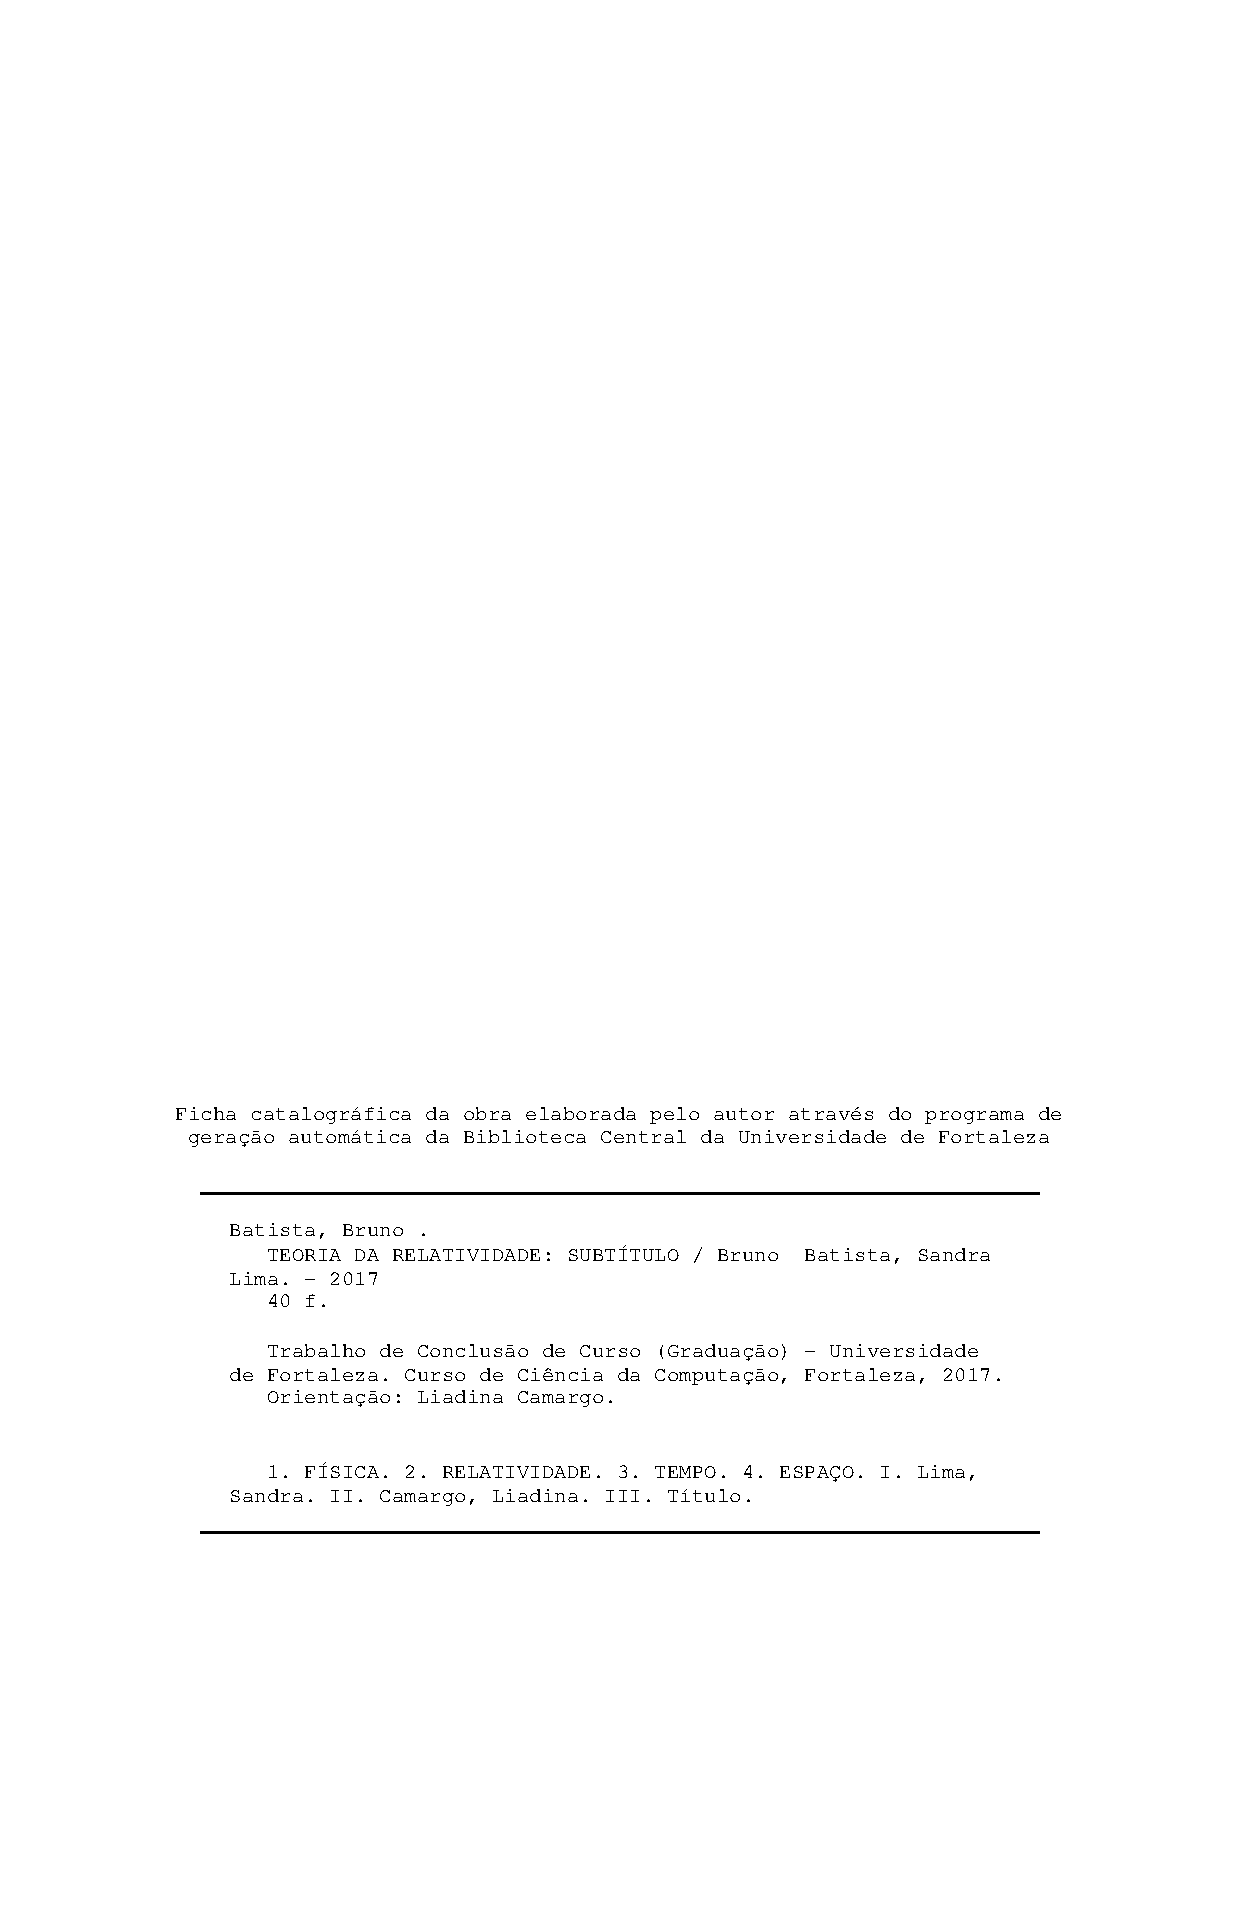
\includepdf{elementos-pre-textuais/folha-aprovacao.pdf}
		\imprimirfolhadeaprovacao

		\imprimirdedicatoria{elementos-pre-textuais/dedicatoria}
		\imprimiragradecimentos{elementos-pre-textuais/agradecimentos}
		\imprimirepigrafe{elementos-pre-textuais/epigrafe}
		\imprimirresumo{elementos-pre-textuais/resumo}
		\imprimirabstract{elementos-pre-textuais/abstract}
	\fi

	% Listas e sumário (comuns aos dois modos; cada lista sai vazia se o
	% documento não tiver o elemento correspondente).
	\imprimirlistadeilustracoes
	\imprimirlistadetabelas
	\imprimirlistadequadros
	\imprimirlistadealgoritmos
	\imprimirlistadecodigosfonte
	\imprimirlistadeabreviaturasesiglas
	\imprimirlistadesimbolos{elementos-pre-textuais/lista-de-simbolos}
	\imprimirsumario

	% Elementos textuais
	\textual
	\ifprobatorio
		%% --- Corpo do Relatório de Comprovação de Período Probatório ---
		%% A Seção 1 (Identificação) é gerada a partir dos metadados do servidor
		%% (\autor, \matriculasiape, \cargo, \lotacao, \periodoprobatorio, \chefia).
		\imprimiridentificacao
		%% >>> A PARTIR DAQUI, adicione os capítulos do SEU relatório. <<<
		%% A Seção 1.2 (entregas do plano de trabalho) e as Seções 2 a 8 são
		%% conteúdo seu: crie os arquivos em elementos-textuais/ e inclua-os com
		%% \input. Esqueleto sugerido (descomente e crie cada arquivo):
		%	\input{elementos-textuais/probatorio/entregas}            % 1.2
		%	\input{elementos-textuais/probatorio/contexto-objetivo}   % 2
		%	\input{elementos-textuais/probatorio/metodologia}         % 3
		%	\input{elementos-textuais/probatorio/comentarios-madeira} % 4
		%	\input{elementos-textuais/probatorio/comentarios-castanha}% 5
		%	\input{elementos-textuais/probatorio/analise-comparativa} % 6
		%	\input{elementos-textuais/probatorio/produtos-entregues}  % 7
		%	\input{elementos-textuais/probatorio/conclusao}           % 8
		%% Bloco de assinatura final (servidor + "De acordo" da chefia):
		\imprimirassinaturas
	\else
		%% >>> SEUS CAPÍTULOS — adicione/remova linhas \input conforme o seu
		%% documento (cada arquivo em elementos-textuais/ começa com \chapter). <<<
		\chapter{Introdução}
\label{cap:introducao}

% Descreva aqui o contexto geral do trabalho, apresentando o tema,
% a problemática e a justificativa da pesquisa.

% [Insira o texto da introdução aqui]
O avanço do conhecimento científico depende, em grande medida, da capacidade de organizar e comunicar resultados de forma clara e padronizada. Instituições de pesquisa como a \gls{EMBRAPA} desempenham papel fundamental nesse processo, ao gerar e difundir conhecimento aplicado a diversos setores, entre eles o da \gls{agropecuaria}. Este documento apresenta, de maneira genérica, a estrutura típica de um trabalho técnico-científico, com o objetivo de demonstrar a formatação adotada pelo template, cujo documento final é gerado em formato \gls{PDF}.

\section{Justificativa}
\label{sec:justificativa}

% Apresente a relevância e a motivação para a realização deste trabalho.

% [Insira a justificativa aqui]
A escolha do tema justifica-se por sua relevância teórica e prática, bem como pela necessidade de aprofundar a compreensão sobre o assunto. A realização deste estudo contribui para preencher lacunas identificadas na literatura e para fornecer subsídios a futuras investigações e aplicações.

\section{Objetivos}
\label{sec:objetivos}

% Apresente os objetivos geral e específicos do trabalho.

\subsection{Objetivo Geral}
\label{sec:objetivo-geral}

% [Insira o objetivo geral aqui]
Investigar de forma sistemática os fatores associados ao problema em estudo, com vistas a ampliar o conhecimento disponível sobre o tema.

\subsection{Objetivos Específicos}
\label{sec:objetivos-especificos}

% Liste os objetivos específicos usando alíneas:
%
% \begin{alineas}
% 	\item Objetivo específico 1;
% 	\item Objetivo específico 2;
% 	\item Objetivo específico 3.
% \end{alineas}

% [Insira os objetivos específicos aqui]
Para alcançar o objetivo geral, foram definidos os seguintes objetivos específicos:

\begin{alineas}
	\item revisar a literatura pertinente ao tema investigado;
	\item descrever os procedimentos metodológicos adotados;
	\item analisar os dados obtidos e discutir os resultados;
	\item apresentar conclusões e recomendações para trabalhos futuros.
\end{alineas}
		\chapter{Revisão de Literatura}
\label{cap:revisao-de-literatura}

% Apresente aqui a fundamentação teórica do trabalho.
% Realize uma revisão bibliográfica dos principais conceitos,
% teorias e trabalhos anteriores relacionados ao tema.

% [Insira o texto da revisão de literatura aqui]
A fundamentação teórica deste trabalho apoia-se em contribuições consolidadas na literatura. De acordo com \citeonline{exemplo-livro}, os conceitos fundamentais que norteiam a área foram estabelecidos a partir de investigações sistemáticas conduzidas ao longo das últimas décadas. Estudos posteriores ampliaram essa compreensão, agregando novas perspectivas ao debate~\cite{exemplo-artigo}.

\section{Tema A}
\label{sec:tema-a}

% [Insira o conteúdo da primeira seção aqui]
Esta seção apresenta os principais conceitos relacionados ao primeiro eixo temático do estudo. A \autoref{fig:exemplo} ilustra, a título de demonstração, uma figura inserida conforme o padrão do template.

\begin{figure}[!htbp]
    \centering
    \EMBRAPAfig{
        \Caption{\label{fig:exemplo} Exemplo de figura inserida com o template}
    }{
        
\includegraphics[width=10cm]{figuras/exemplo_imagem.jpg}
    }{
        \Fonte{Embrapa}
    }
\end{figure}

% Dica: Para inserir uma figura, use o seguinte modelo:
%
% \begin{figure}[!htbp]
%     \centering
%     \EMBRAPAfig{
%         \Caption{\label{fig:modelo} Legenda da figura}
%     }{
%         \includegraphics[width=8cm]{figuras/nome-da-figura}
%     }{
%         \Fonte{Elaborado pelo autor}
%     }
% \end{figure}

\section{Tema B}
\label{sec:tema-b}

% [Insira o conteúdo da segunda seção aqui]
O segundo eixo temático complementa a discussão anterior, abordando aspectos adicionais relevantes para a compreensão do problema. A literatura registra convergências e divergências entre os autores, o que evidencia a riqueza e a complexidade do tema.

% Dica: Para inserir uma tabela, use o seguinte modelo:
%
% \begin{table}[!htbp]
%     \centering
%     \Caption{\label{tab:exemplo} Legenda da tabela}
%     \EMBRAPAtab{}{
%         \begin{tabular}{cll}
%             \toprule
%             Coluna 1 & Coluna 2 & Coluna 3 \\
%             \midrule \midrule
%             Dado 1 & Dado 2 & Dado 3 \\
%             \bottomrule
%         \end{tabular}
%     }{
%         \Fonte{Elaborado pelo autor}
%     }
% \end{table}

		\chapter{Estado da Arte}
\label{cap:estado-da-arte}

% Apresente aqui uma revisão dos trabalhos e pesquisas mais recentes
% relacionados ao tema, destacando as contribuições e lacunas existentes.

% [Insira o texto do estado da arte aqui]
Esta seção apresenta uma síntese dos trabalhos mais recentes relacionados ao tema, com destaque para suas contribuições e para as lacunas ainda existentes.

\section{Trabalho/Pesquisa A}
\label{sec:trabalho-a}

% [Descreva o primeiro trabalho relacionado]
O primeiro trabalho analisado propõe uma abordagem inovadora para o problema, apresentando resultados promissores em cenários controlados.

\section{Trabalho/Pesquisa B}
\label{sec:trabalho-b}

% [Descreva o segundo trabalho relacionado]
O segundo trabalho, por sua vez, adota uma estratégia distinta, privilegiando a generalização dos resultados. O \autoref{qua:comparativo} sintetiza a comparação entre as duas abordagens.

\begin{quadro}[!htbp]
    \centering
    \Caption{\label{qua:comparativo} Comparação entre as abordagens analisadas}
    \EMBRAPAqua{}{
        \begin{tabular}{|l|c|c|}
            \hline
            \textbf{Critério} & \textbf{Trabalho A} & \textbf{Trabalho B} \\
            \hline
            Abordagem & Inovadora & Tradicional \\
            \hline
            Escopo & Restrito & Amplo \\
            \hline
            Desempenho & Alto & Moderado \\
            \hline
        \end{tabular}
    }{
        \Fonte{Elaborado pelo autor}
    }
\end{quadro}

% Dica: Para inserir um quadro comparativo, use o seguinte modelo:
%
% \begin{quadro}[!htbp]
%     \centering
%     \Caption{\label{qua:modelo} Legenda do quadro}
%     \EMBRAPAqua{}{
%         \begin{tabular}{|c|c|c|}
%             \hline
%             Critério & Trabalho A & Trabalho B \\
%             \hline
%             Critério 1 & Valor & Valor \\
%             \hline
%         \end{tabular}
%     }{
%         \Fonte{Elaborado pelo autor}
%     }
% \end{quadro}

		\chapter{Material e Métodos}
\label{cap:material-e-metodos}

% Descreva aqui os materiais utilizados e os métodos empregados
% na realização da pesquisa. Inclua informações sobre:
% - Área de estudo / local do experimento
% - Materiais e equipamentos
% - Delineamento experimental
% - Procedimentos analíticos
% - Análises estatísticas

% [Insira o texto de material e métodos aqui]
Este capítulo descreve os materiais e os métodos empregados na condução do estudo. A apresentação segue as recomendações da \gls{ABNT}, de modo a assegurar a padronização e a reprodutibilidade dos procedimentos.

\section{Área de Estudo}
\label{sec:area-de-estudo}

% [Descreva a área ou local onde o trabalho foi realizado]
O estudo foi conduzido em ambiente representativo do contexto investigado, selecionado de acordo com critérios previamente definidos.

\section{Procedimentos Metodológicos}
\label{sec:procedimentos-metodologicos}

% [Descreva os procedimentos utilizados]
Os procedimentos adotados são sintetizados no \autoref{alg:exemplo}, que descreve, em alto nível, as etapas executadas ao longo do estudo.

\begin{algorithm}[!htbp]
    \SetSpacedAlgorithm
    \caption{\label{alg:exemplo}Procedimento geral adotado no estudo}
    \Entrada{Conjunto de dados brutos $D$}
    \Saida{Resultados consolidados $R$}
    \Inicio{
        \Para{cada elemento $d \in D$}{
            processar $d$\;
            armazenar o resultado parcial\;
        }
        consolidar os resultados em $R$\;
        \Retorna $R$\;
    }
\end{algorithm}

% Dica: Para inserir um algoritmo, use o seguinte modelo:
%
% \begin{algorithm}[h!]
%     \SetSpacedAlgorithm
%     \caption{\label{alg:modelo}Descrição do Algoritmo}
%     \Entrada{Entrada do Algoritmo}
%     \Saida{Saída do Algoritmo}
%     \Inicio{
%         Passo 1\;
%         Passo 2\;
%     }
% \end{algorithm}

\section{Análise dos Dados}
\label{sec:analise-dos-dados}

% [Descreva como os dados foram analisados]
Os dados foram analisados por meio de procedimentos estatísticos descritivos e inferenciais. A relação entre as variáveis é expressa, de forma simplificada, pela \autoref{eq:modelo}.

\begin{equation}
    \label{eq:modelo}
    y = ax + b
\end{equation}

\noindent onde $y$ representa a variável resposta, $x$ a variável explicativa, e $a$ e $b$ os coeficientes do modelo.

Para a inferência sobre a média populacional $\mu$, adotou-se o nível de significância $\alpha$ e construiu-se o intervalo de confiança a partir do desvio-padrão $\sigma$ e do tamanho da amostra $n$, conforme a \autoref{eq:intervalo}.

\begin{equation}
    \label{eq:intervalo}
    \mu = \bar{x} \pm z_{\alpha/2}\,\frac{\sigma}{\sqrt{n}}
\end{equation}

% Dica: Para inserir uma fórmula matemática numerada e referenciável:
%
% \begin{equation}
%     \label{eq:exemplo}
%     y = ax + b
% \end{equation}
%
% Referencie no texto com \autoref{eq:exemplo} (ou \autoref{sec:area-de-estudo}).

		\chapter{Resultados e Discussão}
\label{cap:resultados-e-discussao}

% Apresente aqui os resultados obtidos na pesquisa e discuta-os
% à luz da literatura revisada. Inclua figuras, tabelas e gráficos
% conforme necessário.

% [Insira os resultados e a discussão aqui]
Este capítulo apresenta os resultados obtidos e discute suas implicações à luz da literatura revisada.

\section{Resultados}
\label{sec:resultados}

% [Apresente os resultados obtidos]
Os principais resultados são apresentados na \autoref{tab:resultados}, que sintetiza os valores observados para as variáveis analisadas.

\begin{table}[!htbp]
    \centering
    \Caption{\label{tab:resultados} Síntese dos resultados obtidos}
    \EMBRAPAtab{}{
        \begin{tabular}{lcc}
            \toprule
            Variável & Valor médio & Desvio-padrão \\
            \midrule \midrule
            Indicador A & 12,5 & 1,3 \\
            Indicador B & 8,7 & 0,9 \\
            Indicador C & 21,4 & 2,1 \\
            \bottomrule
        \end{tabular}
    }{
        \Fonte{Elaborado pelo autor}
    }
\end{table}

\section{Discussão}
\label{sec:discussao}

% [Discuta os resultados à luz da literatura]
Os resultados obtidos são coerentes com as expectativas formuladas e dialogam com os achados relatados na literatura. As pequenas divergências observadas podem ser atribuídas a particularidades do contexto investigado e apontam direções para estudos futuros.

		\chapter{Considerações Finais}
\label{cap:consideracoes-finais}

% Apresente aqui as conclusões do trabalho, retomando os objetivos
% propostos e avaliando se foram alcançados.

% [Insira as considerações finais aqui]
Este trabalho buscou investigar de forma sistemática o problema proposto, retomando os objetivos definidos na introdução e avaliando em que medida foram alcançados.

\section{Contribuições do Trabalho}
\label{sec:contribuicoes-do-trabalho}

% [Descreva as principais contribuições]
Entre as principais contribuições do estudo, destacam-se a sistematização do conhecimento sobre o tema e a proposição de subsídios para aplicações práticas.

\section{Limitações}
\label{sec:limitacoes}

% [Descreva as limitações encontradas]
Como toda investigação, este trabalho apresenta limitações, sobretudo quanto ao escopo e às condições em que foi conduzido, o que deve ser considerado na interpretação dos resultados.

\section{Recomendações e Trabalhos Futuros}
\label{sec:recomendacoes-e-trabalhos-futuros}

% [Apresente recomendações e sugestões para trabalhos futuros]
Recomenda-se, para trabalhos futuros, a ampliação do escopo da análise e a investigação de novas variáveis, de modo a consolidar e generalizar os achados aqui apresentados.

	\fi

	% Elementos pós-textuais
	% Todos abaixo aparecem no PDF SOMENTE quando há conteúdo correspondente;
	% caso contrário, são omitidos automaticamente (sem título em página vazia).

	% Referências: impressas se houver \cite/\citeonline no texto. Para forçar
	% a inclusão de uma obra não citada (ex.: a norma ABNT NBR 14724), adicione
	% \nocite{NBR14724:2005} antes da linha abaixo.
	\imprimirreferencias{elementos-pos-textuais/referencias}

	% Glossário: impresso se algum termo do glossário principal for usado no
	% texto com \gls/\Gls (siglas vão para a Lista de Abreviaturas e Siglas).
	\imprimirglossario

	% Apêndices: passe os \input dentro das chaves. Deixe vazio para omitir.
	\imprimirapendices{%
		\apendice{Exemplo de Apêndice}
\label{ap:exemplo-de-apendice}

% Apêndice é um texto ou documento elaborado pelo autor.
% Adicione aqui o conteúdo do apêndice.

Este apêndice apresenta material complementar elaborado pelo autor, como dados adicionais, formulários ou detalhamentos que apoiam o texto principal sem comprometer a sua fluidez.

% Tabela LONGA (multipágina): use o ambiente \EMBRAPAtablonga, que quebra entre
% páginas e repete o cabeçalho automaticamente. Ao contrário de \EMBRAPAtab, ele
% NÃO vai dentro de um ambiente 'table'. Os argumentos são, na ordem: colunas do
% tabular, legenda (com \label), linha de cabeçalho e texto da fonte. Veja o
% README ("Como inserir uma Tabela longa") e o CLAUDE.md.
\begin{EMBRAPAtablonga}{lrr}{\label{tab:apendice-amostras} Resultados de análise das amostras de solo coletadas (dados fictícios)}{Amostra & pH em água & Matéria orgânica (g/kg)}{Elaborado pelo autor}
	Amostra 001 & 5,3 & 21 \\
	Amostra 002 & 6,6 & 28 \\
	Amostra 003 & 4,9 & 35 \\
	Amostra 004 & 5,2 & 42 \\
	Amostra 005 & 6,5 & 17 \\
	Amostra 006 & 4,8 & 24 \\
	Amostra 007 & 5,1 & 31 \\
	Amostra 008 & 6,4 & 38 \\
	Amostra 009 & 4,7 & 45 \\
	Amostra 010 & 5,0 & 20 \\
	Amostra 011 & 6,3 & 27 \\
	Amostra 012 & 4,6 & 34 \\
	Amostra 013 & 5,9 & 41 \\
	Amostra 014 & 6,2 & 16 \\
	Amostra 015 & 4,5 & 23 \\
	Amostra 016 & 5,8 & 30 \\
	Amostra 017 & 6,1 & 37 \\
	Amostra 018 & 4,4 & 44 \\
	Amostra 019 & 5,7 & 19 \\
	Amostra 020 & 6,0 & 26 \\
	Amostra 021 & 4,3 & 33 \\
	Amostra 022 & 5,6 & 40 \\
	Amostra 023 & 6,9 & 15 \\
	Amostra 024 & 4,2 & 22 \\
	Amostra 025 & 5,5 & 29 \\
	Amostra 026 & 6,8 & 36 \\
	Amostra 027 & 4,1 & 43 \\
	Amostra 028 & 5,4 & 18 \\
	Amostra 029 & 6,7 & 25 \\
	Amostra 030 & 4,0 & 32 \\
	Amostra 031 & 5,3 & 39 \\
	Amostra 032 & 6,6 & 14 \\
	Amostra 033 & 4,9 & 21 \\
	Amostra 034 & 5,2 & 28 \\
	Amostra 035 & 6,5 & 35 \\
	Amostra 036 & 4,8 & 42 \\
	Amostra 037 & 5,1 & 17 \\
	Amostra 038 & 6,4 & 24 \\
	Amostra 039 & 4,7 & 31 \\
	Amostra 040 & 5,0 & 38 \\
\end{EMBRAPAtablonga}
%
	}

	% Anexos: passe os \input dentro das chaves. Deixe vazio para omitir.
	\imprimiranexos{%
		\anexo{Exemplo de Anexo}
\label{an:exemplo-de-anexo}

% Anexo é um texto ou documento não elaborado pelo autor.
% Adicione aqui o conteúdo do anexo.

% [Insira o conteúdo do anexo aqui]
Este anexo reúne material de apoio não elaborado pelo autor, como documentos, tabelas ou normas de terceiros que complementam o conteúdo do trabalho.%
	}

	% Índice remissivo: impresso apenas se houver entradas \index{} no texto.
	\imprimirindice

\end{document}

